% !TEX program = xelatex
% Báo cáo kiến tập - Khoa Hệ thống thông tin, UEL
% Biên dịch: xelatex main.tex (chạy 2 lần để cập nhật mục lục)
\documentclass[a4paper]{article}
\usepackage[fontsize=13pt]{scrextend} % extarticle không có cỡ 13pt; scrextend đặt cỡ chữ bất kỳ

\usepackage{fontspec}
\setmainfont{Times New Roman}
\usepackage[left=3cm,right=2cm,top=2.5cm,bottom=2.5cm]{geometry}
\usepackage{needspace}
\usepackage{setspace,indentfirst,graphicx,float,xcolor,tikz}
\usepackage{array,tabularx,longtable,multirow,enumitem}
\usepackage{titlesec}
\usepackage[font=it,labelsep=colon,justification=centering]{caption}
\usepackage[style=apa,backend=biber]{biblatex}
\addbibresource{references.bib}
\usepackage{fancyhdr}
\pagestyle{plain} % chỉ số trang ở giữa chân trang, không header
\usetikzlibrary{arrows.meta,positioning,shapes.geometric,fit,calc}
\tikzset{
  khoi/.style={draw,rounded corners=2pt,align=center,font=\small,minimum height=8mm,inner sep=4pt},
  quyetdinh/.style={draw,diamond,aspect=2.2,align=center,font=\small,inner sep=1pt},
  mui/.style={-{Stealth[length=2mm]},thick},
  nhan/.style={font=\footnotesize,align=center}}
% Các hình TikZ được dựng theo tọa độ cm với chữ cỡ 10pt. Thân bài 13pt làm chữ trong hình
% to hơn khung và chồng lên nhau, nên bên trong mỗi hình dùng lại bộ cỡ chữ của 10pt.
\tikzset{every picture/.append style={execute at begin picture={%
  \def\small{\fontsize{9}{11}\selectfont}\def\footnotesize{\fontsize{8}{9.5}\selectfont}%
  \def\scriptsize{\fontsize{7}{8}\selectfont}\def\tiny{\fontsize{5}{6}\selectfont}%
  \fontsize{10}{12}\selectfont}}}
\usepackage{listings}
\lstset{basicstyle=\ttfamily\small\linespread{1}\selectfont,breaklines=true,frame=single,columns=fullflexible,showstringspaces=false,upquote=true,
  aboveskip=6pt,belowskip=12pt,framesep=4pt,xleftmargin=4pt,xrightmargin=4pt}
\usepackage[hidelinks,unicode]{hyperref}

% ---------- Thông tin báo cáo (sửa tại đây) ----------
\newcommand{\tenkhoa}{KHOA HỆ THỐNG THÔNG TIN}
\newcommand{\tennganh}{HỆ THỐNG THÔNG TIN QUẢN LÝ}
\newcommand{\tenchuyennganh}{KINH DOANH SỐ VÀ TRÍ TUỆ NHÂN TẠO}
\newcommand{\tendetai}{TRIỂN KHAI TỰ ĐỘNG HÓA, MÔ PHỎNG MCP SERVER VÀ GIÁM SÁT PHÂN QUYỀN AI AGENT QUA MCP GATEWAY}
\newcommand{\gvhd}{PGS.TS. Lê Hoành Sử}
% Nhóm hai sinh viên: bìa dùng từng người (A, B); \svth và \mssv ghép cả hai cho các phiếu
\newcommand{\svthA}{Vòng Hữu Quân}
\newcommand{\mssvA}{K244161803}
\newcommand{\svthB}{Nguyễn Trần Thái Huy}
\newcommand{\mssvB}{K244161784}
\newcommand{\svth}{\svthA{} -- \svthB}
\newcommand{\mssv}{\mssvA{} -- \mssvB}
\newcommand{\lop}{K24416}
\newcommand{\thoigian}{TP.HCM, THÁNG 11/2026}
\newcommand{\coquan}{Công ty Tài chính Tổng hợp cổ phần Tín Việt (VietCredit)}
\newcommand{\mentor}{Đinh Văn An}

% ---------- Trình bày chung ----------
% Bằng "1.5 lines" của Word: dòng đơn TNR = 1,15 x 13pt, nhân 1,5 = 22,4pt; baselineskip gốc 15,6pt
\setstretch{1.4375}
\setlength{\parindent}{1.27cm}
\setlength{\parskip}{6pt}
\setlength{\emergencystretch}{3em} % cho phép giãn khoảng trắng để tên dài trong \texttt không tràn lề
\tolerance=1000
\graphicspath{{images/}}
\renewcommand{\contentsname}{MỤC LỤC}
\renewcommand{\listfigurename}{DANH MỤC HÌNH ẢNH}
\renewcommand{\listtablename}{DANH MỤC BẢNG}
\renewcommand{\figurename}{Hình}
\renewcommand{\tablename}{Bảng}
\counterwithin{figure}{section}
\counterwithin{table}{section}
\captionsetup[table]{position=top}

% ---------- Đề mục ----------
\setcounter{secnumdepth}{4}
\setcounter{tocdepth}{4}
\titleformat{\section}{\centering\bfseries}{}{0pt}{}
\titleformat{\subsection}{\bfseries}{\thesubsection}{0.5em}{}
\titleformat{\subsubsection}{\normalfont}{\thesubsubsection}{0.5em}{} % mẫu của Khoa: 1.1.1 không in đậm
\titleformat{\paragraph}[hang]{\itshape}{\theparagraph}{0.5em}{}
\titlespacing*{\section}{0pt}{0pt}{12pt}
\titlespacing*{\subsection}{0pt}{12pt}{6pt}
\titlespacing*{\subsubsection}{0pt}{12pt}{6pt}
\titlespacing*{\paragraph}{0pt}{6pt}{6pt}

% \heading{...}: đề mục lớn không đánh số (LỜI CẢM ƠN, A., B., C., ...)
\newcommand{\heading}[1]{\clearpage\phantomsection\section*{#1}\addcontentsline{toc}{section}{#1}}
% \phan{...}: "PHẦN n: ..." trong mục B; \phan[]{...} để không sang trang mới
\newcommand{\phan}[2][\clearpage]{#1\refstepcounter{section}%
  \section*{PHẦN \thesection: #2}\addcontentsline{toc}{phan}{PHẦN \thesection: #2}}
% \chuong{...}: "CHƯƠNG n: ..." — cấp cao nhất của nội dung chính (1, 1.1, 1.1.1)
\newcommand{\chuong}[1]{\clearpage\refstepcounter{section}%
  \section*{CHƯƠNG \thesection: #1}\addcontentsline{toc}{section}{CHƯƠNG \thesection: #1}}
% Tiểu mục không đánh số, không vào mục lục
\newcommand{\tieumuc}[1]{\par\textbf{#1}\par}
\newcommand{\tieumucnghieng}[1]{\par\textit{#1}\par}

% ---------- Mục lục ----------
\makeatletter
\renewcommand*\l@section[2]{\addvspace{4pt}\@dottedtocline{1}{0em}{0em}{\bfseries #1}{\bfseries #2}}
\newcommand*\l@phan[2]{\@dottedtocline{1}{0.5cm}{0em}{\bfseries #1}{\bfseries #2}}
\renewcommand*\l@subsection[2]{\@dottedtocline{2}{1cm}{2em}{\bfseries #1}{\bfseries #2}}
\renewcommand*\l@subsubsection{\@dottedtocline{3}{1.5cm}{2.6em}}
\renewcommand*\l@paragraph{\@dottedtocline{4}{3cm}{3.4em}}
\newcommand*\toclevel@phan{1}
\renewcommand\@pnumwidth{2.2em} % đủ chỗ cho số trang La Mã như xviii
\makeatother

% ---------- Tiện ích giữ chỗ (xoá khi viết nội dung thật) ----------
\newcommand{\todo}[1]{\par{\color{gray}\textit{[#1]}}\par}
\newcommand{\nguon}[1]{\par\textit{Nguồn: #1}\par}
% \hinh{chú thích}{nhãn}: thay \fbox bằng \includegraphics
\newcommand{\hinh}[2]{\begin{figure}[H]\centering
  \fbox{\parbox[c][3.5cm][c]{0.7\textwidth}{\centering\color{gray}\textit{[Chèn hình]}}}
  \caption{#1}\label{#2}\end{figure}}
% \bang{chú thích}{nhãn}{số cột}{hàng tiêu đề}
\newcommand{\bang}[4]{\begin{table}[H]\centering\caption{#1}\label{#2}
  \begin{tabularx}{\textwidth}{|*{#3}{>{\centering\arraybackslash}X|}}\hline
  #4 \\ \hline
  \multicolumn{#3}{|c|}{\color{gray}\textit{[Nội dung bảng]}} \\ \hline
  \end{tabularx}\end{table}}
\newcommand{\dongcham}[1]{\par\noindent\foreach \i in {1,...,#1}{\makebox[\textwidth]{\dotfill}\\}\par\bigskip}

\begin{document}

\pagenumbering{roman}
% ===== frontmatter.tex =====
% ================= BÌA =================
\begin{titlepage}
\begin{tikzpicture}[remember picture,overlay]
  \node[inner sep=0] at (current page.center)
    {
\includegraphics[width=\paperwidth,height=\paperheight]{cover-bg.jpg}};
  \node[font=\bfseries\fontsize{18}{24}\selectfont] at ([yshift=-45mm]current page.north) {\tenkhoa};
  \node[font=\bfseries\fontsize{15}{20}\selectfont,align=center] at ([yshift=-123mm]current page.north)
    {BÁO CÁO KIẾN TẬP\\[4pt] NGÀNH \tennganh\\[4pt] (CHUYÊN NGÀNH \tenchuyennganh)};
  \node[font=\bfseries\fontsize{15}{22}\selectfont,align=center,text width=17cm] at ([yshift=-164mm]current page.north) {\tendetai};
  \node[anchor=north,font=\fontsize{14}{20}\selectfont] at ([xshift=30mm,yshift=-194mm]current page.north)
    {\renewcommand{\arraystretch}{1.0}\begin{tabular}{@{}l@{\hspace{3mm}}l@{\hspace{8mm}}l@{\hspace{2mm}}l@{}}
     \textbf{GVHD:} & \multicolumn{3}{l}{\gvhd}\\
     \textbf{SVTH:} & \svthA & \textbf{MSSV:} & \mssvA\\
                    & \svthB & \textbf{MSSV:} & \mssvB
     \end{tabular}};
  \node[font=\bfseries,text=white] at ([yshift=-271mm]current page.north) {\thoigian};
\end{tikzpicture}
\end{titlepage}
\setcounter{page}{1}

% ================= LỜI CẢM ƠN =================
\heading{LỜI CẢM ƠN}
Nhóm xin cảm ơn Khoa Hệ thống thông tin, Trường Đại học Kinh tế -- Luật đã tổ chức học phần kiến tập, giúp sinh viên được làm việc tại doanh nghiệp ngay trong quá trình học.

Nhóm xin cảm ơn \gvhd{}, giảng viên hướng dẫn, đã nhận hướng dẫn nhóm và dành thời gian đọc, góp ý cho đề tài cũng như cho bản báo cáo này.

Nhóm xin cảm ơn \coquan{} đã tiếp nhận nhóm kiến tập, và cảm ơn người hướng dẫn tại đơn vị, anh \mentor, đã định hướng và hỗ trợ nhóm trong suốt thời gian kiến tập. Đề tài bắt nguồn từ một nhu cầu rất cụ thể của nhóm dữ liệu, đó là cho AI Agent dùng công cụ trên Kubernetes, Spark, OpenMetadata, dbt và Airflow mà vẫn biết rõ agent nào được làm gì và đã làm gì. Bài toán ấy dạy nhóm một thói quen. Trước mỗi quy tắc cấu hình, nhóm tự hỏi nếu viết sai cấu hình thì agent nào sẽ nhận quyền mà nó không nên có.

Sản phẩm trong báo cáo là bản chứng minh khái niệm chạy trên một cụm Kubernetes cục bộ, và chưa được triển khai lên máy chủ thật. Nhóm mong tiếp tục nhận được góp ý của giảng viên hướng dẫn và đơn vị để hoàn thiện đề tài.

\vspace{12pt}
\hfill\begin{minipage}{10cm}\centering
TP. Hồ Chí Minh, ngày 11 tháng 11 năm 2026\\
\textbf{Nhóm sinh viên thực hiện}\\[4pt]
\svthA\\
\svthB
\end{minipage}

% ================= LỜI CAM KẾT =================
\heading{LỜI CAM KẾT}
Nhóm sinh viên xin cam kết báo cáo kiến tập này là kết quả làm việc của chính nhóm trong thời gian kiến tập tại \coquan, dưới sự hướng dẫn của \gvhd{} và người hướng dẫn tại đơn vị \mentor. Các số liệu và kết quả kiểm chứng trong báo cáo được thu thập từ môi trường thử nghiệm do nhóm tự dựng, trung thực và chưa từng được công bố trong bất kỳ báo cáo nào khác. Những nội dung tham khảo từ tài liệu, công trình của tác giả khác đều được trích dẫn đầy đủ trong danh mục tài liệu tham khảo. Báo cáo không sử dụng dữ liệu nghiệp vụ hay thông tin bảo mật của đơn vị kiến tập. Nhóm xin chịu hoàn toàn trách nhiệm về nội dung của báo cáo.

\vspace{12pt}
\hfill\begin{minipage}{10cm}\centering
TP. Hồ Chí Minh, ngày 11 tháng 11 năm 2026\\
\textbf{Nhóm sinh viên thực hiện}\\[4pt]
\svthA\\
\svthB
\end{minipage}

% ================= PHIẾU ĐÁNH GIÁ KẾT QUẢ KIẾN TẬP =================
\clearpage
\section*{PHIẾU ĐÁNH GIÁ KẾT QUẢ KIẾN TẬP}
{\setlength{\parskip}{0pt}\singlespacing
MSSV: \mssvB

Họ tên: \svthB

Tên Cơ quan Kiến tập: \coquan

Địa chỉ Cơ quan: 43-45 Thảo Điền, An Khánh, thành phố Hồ Chí Minh

Điện thoại Cơ quan: 1900638996

Họ tên người đại diện cơ quan: \mentor

Chức vụ: chuyên viên Quản trị Dữ liệu \quad Điện thoại: 0328783611

Thời gian kiến tập tại Cơ quan: Từ ngày 27/09/2026 Đến ngày: 04/11/2026

\textit{* Đề nghị \textbf{Quý Cơ quan} đánh giá \textbf{bằng cách đánh dấu X} vào cột xếp loại các nội dung đánh giá trong bảng sau.}

Ghi chú:

\textbf{\textit{Loại A: 2đ; Loại B: 1,5đ}}

\textbf{\textit{Loại C: 1đ; Loại D: 0,5đ}}
\par}
\vspace{6pt}
{\singlespacing\renewcommand{\arraystretch}{1.4}\noindent
\begin{tabularx}{\textwidth}{|X|c|c|c|c|}\hline
\multirow{2}{*}{\centering\textbf{Nội dung đánh giá}} & \multicolumn{4}{c|}{\textbf{Xếp loại}} \\ \cline{2-5}
 & \makebox[0.8cm]{A} & \makebox[0.8cm]{B} & \makebox[0.8cm]{C} & \makebox[0.8cm]{D} \\ \hline
\multicolumn{5}{|l|}{\textbf{1. Tinh thần kỷ luật, thái độ}} \\ \hline
\quad 1.1 Thực hiện nội quy của cơ quan & X & & & \\ \hline
\quad 1.2 Chấp hành giờ giấc làm việc & X & & & \\ \hline
\quad 1.3 Thái độ giao tiếp với đồng nghiệp, cộng sự & X & & & \\ \hline
\quad 1.4 Ý thức bảo vệ tài sản & X & & & \\ \hline
\quad 1.5 Tích cực trong công việc & X & & & \\ \hline
\multicolumn{5}{|l|}{\textbf{2. Kỹ năng chuyên môn, nghiệp vụ}} \\ \hline
\quad 2.1 Đáp ứng yêu cầu công việc & X & & & \\ \hline
\quad 2.2 Tinh thần học hỏi, nâng cao trình độ chuyên môn & X & & & \\ \hline
\quad 2.3 Có sáng kiến, năng động trong công việc & X & & & \\ \hline
\multicolumn{5}{|l|}{\textbf{3. Kết quả thực tập}} \\ \hline
\quad 3.1 Có sản phẩm ứng dụng thực tế đem lại lợi ích cho Cơ quan & X & & & \\ \hline
\quad 3.2 Mức độ hoàn thành nhiệm vụ thực tập & X & & & \\ \hline
\end{tabularx}}

% ================= PHIẾU NHẬN XÉT CƠ QUAN KIẾN TẬP =================
\clearpage
\section*{PHIẾU NHẬN XÉT CƠ QUAN KIẾN TẬP}
Huy có tinh thần học hỏi tốt, có trách nhiệm cao trong công việc. Đối với các bài toán, kiến thức mới ngoài phạm vi hiểu biết hiện tại, bạn đã chủ động tìm hiểu, tham vấn ý kiến từ người hướng dẫn và tiếp nhận rất nhanh. Trong thời gian ngắn, bạn đã triển khai đầy đủ các tính năng cốt lõi của sản phẩm, đáp ứng được nhu cầu thực tế về phân quyền và bảo mật dữ liệu trong việc quản trị MCP theo vai trò của từng người và agent trong doanh nghiệp. Tôi đánh giá cao những gì Huy đã làm, đã đóng góp cho công ty trong thời gian kiến tập vừa qua.
\vspace{12pt}

\hfill\begin{minipage}{8cm}\centering
TP HCM, ngày 12 tháng 11 năm 2026.\\
\textbf{XÁC NHẬN CỦA CƠ QUAN}\\
\textit{Ký, ghi rõ họ tên, đóng dấu}\\[4pt]
\includegraphics[width=5cm]{chu-ky-co-quan.jpg}
\end{minipage}

% ================= PHIẾU ĐÁNH GIÁ CỦA GVHD =================
\clearpage
\section*{PHIẾU ĐÁNH GIÁ BÁO CÁO KIẾN TẬP\\ CỦA GIẢNG VIÊN HƯỚNG DẪN}
{\setlength{\parskip}{0pt}\singlespacing
MSSV: \mssv

Họ tên: \svth

Lớp: \lop

Ngành/Chuyên ngành: \tennganh{} (Chuyên ngành \tenchuyennganh)

Tên đề tài: \tendetai

GVHD: \gvhd
\par}
\vspace{6pt}
{\singlespacing\renewcommand{\arraystretch}{1.3}\noindent
\begin{tabularx}{\textwidth}{|c|>{\centering\arraybackslash}X|c|>{\centering\arraybackslash}p{2.2cm}|}\hline
\textbf{STT} & \textbf{Tiêu chí cụ thể} & \textbf{Tỉ lệ} & \textbf{Điểm đã nhân tỉ lệ} \\ \hline
1 & Tuân thủ quy định học phần, đúng tiến độ, đầy đủ xác nhận của đơn vị/leader, tinh thần học tập nghiêm túc & 10\% & \\ \hline
2 & Tìm hiểu doanh nghiệp, môi trường làm việc, vị trí nghề nghiệp, xác định định hướng chuyên sâu rõ ràng & 10\% & \\ \hline
3 & Mô tả bối cảnh thực tế, xác định vấn đề/tình huống rõ ràng, có logic và phù hợp với định hướng nghề nghiệp & 15\% & \\ \hline
4 & Vận dụng kiến thức chuyên ngành, kiến thức kinh doanh quản lý, công nghệ để phân tích vấn đề & 20\% & \\ \hline
5 & Thu thập dữ liệu, xử lý dữ liệu, phân tích, diễn giải kết quả, sử dụng bảng biểu/hình minh họa phù hợp & 15\% & \\ \hline
6 & Đề xuất giải pháp phù hợp, có tính ứng dụng, khả thi trong bối cảnh thực tế & 15\% & \\ \hline
7 & Bố cục logic, trình bày khoa học, ngôn ngữ học thuật, trích dẫn tài liệu, hình thức đúng quy định & 15\% & \\ \hline
\multicolumn{3}{|c|}{Tổng điểm:} & \\[12pt] \hline
\end{tabularx}}

\vspace{6pt}
\hfill\begin{minipage}{8cm}\centering
............, ngày ..... tháng ..... năm .......\\
\textbf{Giảng viên hướng dẫn}\\
\textit{Ký, ghi rõ họ tên}
\end{minipage}

% ================= PHIẾU NHẬN XÉT CỦA GVHD =================
\clearpage
\section*{PHIẾU NHẬN XÉT CỦA GIẢNG VIÊN HƯỚNG DẪN}
\dongcham{19}
\vspace{6pt}
\hfill\begin{minipage}{8cm}\centering
............, ngày ..... tháng ..... năm .......\\
\textbf{Giảng viên hướng dẫn}\\
\textit{Ký, ghi rõ họ tên}
\end{minipage}

% ================= LỊCH LÀM VIỆC =================
\heading{LỊCH LÀM VIỆC VÀ NỘI DUNG CÔNG VIỆC}
{\singlespacing\small\renewcommand{\arraystretch}{1.3}
\begin{longtable}{|c|>{\raggedright\arraybackslash}p{2.2cm}|>{\raggedright\arraybackslash}p{6.9cm}|>{\raggedright\arraybackslash}p{4.0cm}|}\hline
\textbf{Tuần} & \textbf{Thời gian (2026)} &\textbf{Nội dung công việc} & \textbf{Sản phẩm / minh chứng} \\ \hline
\endhead
Chuẩn bị & 12/09 đến 26/09 & Khởi tạo kho mã. Tìm hiểu đặc tả MCP, so sánh các phương án MCP gateway (IBM ContextForge, agentgateway, Azure API Management) và viết bản hướng dẫn triển khai đầu tiên. & Commit \texttt{932f919}, báo cáo nghiên cứu trong \path{local-docs/} \\ \hline
1 & 27/09 đến 02/10 & Dựng khung thư mục theo phương án ban đầu dùng ContextForge, gồm chỗ cho các mock server theo nhóm nghiệp vụ và bảng ánh xạ nhóm với công cụ ở dạng nháp. Tìm hiểu agentgateway, Gateway API và chạy thử trên kind. & Commit \texttt{7e7dcb7} \\ \hline
2 & 03/10 đến 09/10 & Chuyển sang agentgateway và bỏ khung ContextForge. Dựng Gateway, HTTPRoute và backend hợp nhất năm target; viết năm mock MCP server và kiểm thử gọi đủ 21 công cụ qua gateway. Rà soát access log, metric, trace và lệnh gọi bị từ chối. Triển khai Keycloak, xác thực JWT và bản đầu của chính sách phân quyền theo công cụ. & \path{deploy/agentgateway/}, \path{servers/}, \path{evidence/gateway-smoke.txt}, \path{rbac/tool-access.yaml} \\ \hline
3 & 10/10 đến 16/10 & Bổ sung bản phần mềm thật cho radar, OpenMetadata và Spark History chạy song song với mock, giữ nguyên tên target; thêm NetworkPolicy, thiết kế token exchange cho OpenMetadata và kiểm thử bằng curl, MCP Inspector. Viết \texttt{run.sh}, \texttt{bootstrap.sh}, \texttt{QUICKSTART.md}, script xóa cụm \texttt{ops/down.ps1} và dashboard Grafana allow/deny. Dựng khung báo cáo LaTeX đầu tiên. & \path{deploy/real-servers/}, \path{deploy/network/}, \path{ops/down.ps1}, \path{observability/grafana/} \\ \hline
4 và 5 & 17/10 đến 30/10 & Chuyển trọng tâm sang danh tính AI Agent, trong đó mỗi agent là một client Keycloak riêng và nhận vai trò năng lực qua claim \texttt{roles}. Cập nhật xác thực JWT, phân quyền và access log theo agent; viết ma trận agent, vai trò và công cụ dạng JSON, kiểm thử \texttt{agent\_rbac\_smoke.py} và kiểm thử tĩnh đối chiếu cấu hình. & \path{deploy/keycloak/realm-config.yaml}, \path{tests/expected/agent-tool-access.json}, \path{evidence/agent-rbac-smoke.txt} \\ \hline
6 & 31/10 đến 04/11 & Hợp nhất nhánh \texttt{dev}, gộp persona người dùng với vai trò AI Agent, thêm \texttt{ops/up.ps1} và script nạp agent vào realm. Vẽ sơ đồ kiến trúc, chụp dashboard allow/deny và đo thời gian khởi động. Viết các chương báo cáo và đối chiếu nội dung với kho mã. & \path{ops/up.ps1}, \path{deploy/keycloak/setup-agents.sh}, \path{docs/diagrams/}, \path{evidence/ops-up-timing.txt}, \path{report/} \\ \hline
\end{longtable}}

% ================= MỤC LỤC & CÁC DANH MỤC =================
\clearpage\phantomsection
\addcontentsline{toc}{section}{MỤC LỤC}
{\setlength{\parskip}{0pt}\tableofcontents}

\clearpage\phantomsection
\addcontentsline{toc}{section}{DANH MỤC HÌNH ẢNH}
{\setlength{\parskip}{0pt}\renewcommand{\numberline}[1]{Hình #1: }\listoffigures}

\clearpage\phantomsection
\addcontentsline{toc}{section}{DANH MỤC BẢNG}
{\setlength{\parskip}{0pt}\renewcommand{\numberline}[1]{Bảng #1: }\listoftables}

\heading{DANH MỤC TỪ VIẾT TẮT}
{\singlespacing\renewcommand{\arraystretch}{1.5}
\begin{longtable}{|>{\centering\arraybackslash}p{2.2cm}|>{\centering\arraybackslash}p{6.1cm}|>{\centering\arraybackslash}p{6.1cm}|}\hline
\textbf{Từ viết tắt} & \textbf{Cụm từ đầy đủ} & \textbf{Diễn giải} \\ \hline
\endhead
AI & Artificial Intelligence & Trí tuệ nhân tạo \\ \hline
API & Application Programming Interface & Giao diện lập trình ứng dụng \\ \hline
CEL & Common Expression Language & Ngôn ngữ biểu thức của chính sách \\ \hline
CI/CD & Continuous Integration / Continuous Delivery & Tích hợp và triển khai liên tục \\ \hline
CRD & Custom Resource Definition & Tài nguyên tùy biến của Kubernetes \\ \hline
DAG & Directed Acyclic Graph & Đồ thị có hướng không chu trình, đơn vị luồng công việc của Airflow \\ \hline
HTTP & Hypertext Transfer Protocol & Giao thức truyền siêu văn bản \\ \hline
IaC & Infrastructure as Code & Quản lý hạ tầng bằng mã \\ \hline
IP & Internet Protocol & Giao thức Internet \\ \hline
JSON & JavaScript Object Notation & Định dạng dữ liệu dạng văn bản \\ \hline
JSON-RPC & JSON Remote Procedure Call & Giao thức gọi thủ tục từ xa mã hóa bằng JSON \\ \hline
JWKS & JSON Web Key Set & Tập khóa công khai dùng để xác minh JWT \\ \hline
JWS & JSON Web Signature & Chữ ký số cho dữ liệu JSON \\ \hline
JWT & JSON Web Token & Mã thông báo dạng JSON \\ \hline
MCP & Model Context Protocol & Giao thức ngữ cảnh mô hình \\ \hline
NHNN & Ngân hàng Nhà nước Việt Nam & State Bank of Vietnam \\ \hline
NIST & National Institute of Standards and Technology & Viện Tiêu chuẩn và Công nghệ Quốc gia Hoa Kỳ \\ \hline
OAuth & Open Authorization & Khung chuẩn ủy quyền truy cập \\ \hline
OIDC & OpenID Connect & Giao thức xác thực trên OAuth 2.0 \\ \hline
RBAC & Role-Based Access Control & Kiểm soát truy cập theo vai trò \\ \hline
RFC & Request for Comments & Văn bản đặc tả chuẩn của IETF \\ \hline
SDK & Software Development Kit & Bộ công cụ phát triển phần mềm \\ \hline
SSE & Server-Sent Events & Luồng sự kiện máy chủ đẩy về client \\ \hline
UPCoM & Unlisted Public Company Market & Thị trường giao dịch cổ phiếu của công ty đại chúng chưa niêm yết \\ \hline
WSL & Windows Subsystem for Linux & Môi trường Linux chạy trên Windows \\ \hline
\end{longtable}}

\heading{DANH MỤC THUẬT NGỮ}
{\singlespacing\renewcommand{\arraystretch}{1.5}
\begin{longtable}{|>{\centering\arraybackslash}p{1.5cm}|>{\centering\arraybackslash}p{6.2cm}|>{\centering\arraybackslash}p{6.9cm}|}\hline
\textbf{STT} & \textbf{Thuật ngữ gốc} & \textbf{Ý nghĩa} \\ \hline
\endhead
1 & AI Agent & Tác tử AI tự gọi công cụ để hoàn thành tác vụ \\ \hline
2 & MCP Gateway & Cổng tập trung xác thực, phân quyền, định tuyến MCP \\ \hline
3 & Tool & Hàm mà MCP server cung cấp cho tác tử \\ \hline
4 & Mock server & Máy chủ giả lập trả dữ liệu mẫu \\ \hline
5 & Deny-by-default & Mặc định từ chối, chỉ cho phép khi có quy tắc \\ \hline
6 & Observability & Khả năng quan sát qua log, metric, trace \\ \hline
7 & Access log & Nhật ký truy cập \\ \hline
8 & Target & Một MCP server phía sau gateway; tên target là tiền tố của tên công cụ \\ \hline
9 & Multiplexing & Gộp danh mục công cụ của nhiều server thành một \\ \hline
10 & Client credentials & Luồng OAuth 2.0 để client tự xin token nhân danh chính nó \\ \hline
11 & Token exchange & Đổi token đang có lấy token dành cho một dịch vụ cụ thể \\ \hline
12 & Policy attachment & Mẫu gắn chính sách vào tài nguyên của Gateway API \\ \hline
13 & Idempotent & Chạy một hay nhiều lần đều cho cùng kết quả \\ \hline
\end{longtable}}
\clearpage\pagenumbering{arabic} % trang 1 bắt đầu từ Chương 1
% ===== chapters/ch1-don-vi.tex =====
\chuong{TỔNG QUAN VỀ ĐƠN VỊ KIẾN TẬP}

Chương này giới thiệu đơn vị kiến tập theo ba lớp, đi từ rộng đến hẹp. Lớp ngoài cùng là công ty và lĩnh vực hoạt động, kế đến là bộ phận nơi nhóm làm việc, sau cùng là vị trí của nhóm trong bộ phận ấy. Qua ba lớp này, chương muốn cho thấy bài toán kiểm soát truy cập của AI Agent, vốn là chủ đề của các chương sau, xuất phát từ nhu cầu có thật của một công ty tài chính.

\subsection{Giới thiệu Công ty Tài chính Tổng hợp cổ phần Tín Việt}

\subsubsection{Lịch sử hình thành}

Đơn vị kiến tập là Công ty Tài chính Tổng hợp cổ phần Tín Việt (VietCredit General Finance Joint Stock Company, gọi tắt là VietCredit). Công ty được Ngân hàng Nhà nước Việt Nam (NHNN) cấp phép năm 2008 với tên Công ty Tài chính cổ phần Xi măng \parencite{vietcredit_bctn2025}. Mười năm sau, ngày 18/6/2018, NHNN cấp đổi giấy phép và công ty mang tên Công ty Tài chính cổ phần Tín Việt; thời điểm đó vốn điều lệ vào khoảng 605 tỷ đồng, và Tổng công ty Công nghiệp Xi măng Việt Nam (Vicem) là cổ đông lớn duy nhất \parencite{nhadautu_doiten2018}. Cũng từ năm 2018, công ty rẽ sang mảng tài chính tiêu dùng \parencite{vietcredit_bctn2025}. Chữ ``Tổng hợp'' trong tên hiện tại chỉ xuất hiện từ ngày 26/05/2025 \parencite{baodautu_doiten2025}.

Tính đến ngày 31/12/2025, VietCredit có vốn điều lệ khoảng 912 tỷ đồng và 454 cán bộ nhân viên. Trụ sở chính đặt tại Hà Nội, kèm một chi nhánh tại Thành phố Hồ Chí Minh, và cổ phiếu của công ty giao dịch trên UPCoM với mã TIN \parencite{vietcredit_bctn2025}.

\subsubsection{Lĩnh vực hoạt động}

Với tư cách công ty tài chính tổng hợp, VietCredit được huy động vốn, cấp tín dụng dưới các hình thức cho vay tiêu dùng, phát hành thẻ tín dụng và cho thuê tài chính, đồng thời cung cấp một số dịch vụ tài chính khác trong phạm vi giấy phép của NHNN \parencite{vietcredit_bctn2025}. Trên thực tế, trọng tâm là cho vay qua kênh số. Sản phẩm Tin Vay được nhúng vào ứng dụng của các đối tác như MoMo, Viettel Money, Zalo và Grab, nhờ vậy khách hàng vay hoàn toàn trực tuyến; song song có Tin Vay Biz dành cho hộ kinh doanh và nền tảng TIN GO cho vay mua xe điện. Đến cuối năm 2025, gần 80\% dư nợ đến từ cho vay qua công nghệ số \parencite{vietcredit_kqkd2025}. Quy mô vẫn tăng nhanh. Ngày 30/9/2026, dư nợ cho vay khách hàng chạm gần 20.928 tỷ đồng, cao hơn cùng kỳ trên 124\%, còn lợi nhuận trước thuế chín tháng đầu năm 2026 đạt 1.558,6 tỷ đồng \parencite{vnba_9t2026}.

Khi gần như toàn bộ hoạt động cho vay vận hành trên hệ thống, an toàn thông tin trở thành điều kiện để kinh doanh chứ không còn là việc riêng của bộ phận kỹ thuật. Báo cáo thường niên ghi rằng các hệ thống thông tin của công ty được phân loại từ cấp độ 1 đến cấp độ 3 theo quy định của NHNN, mỗi cấp độ đi kèm biện pháp bảo mật tương ứng; cùng lúc, công ty đặt chuyển đổi số, trong đó có trí tuệ nhân tạo và tự động hóa, làm trọng tâm chiến lược năm 2026 \parencite{vietcredit_bctn2025}. Hai định hướng ấy gặp nhau ở câu hỏi mà đề tài theo đuổi. Một AI Agent được phép thao tác trên những hệ thống đã phân cấp bảo mật thì phải chịu cùng khuôn khổ kiểm soát truy cập như một nhân viên.

\subsubsection{Quy trình làm việc}

Trong phạm vi đề tài, quy trình làm việc của nhóm có thể truy lại qua lịch sử kho mã. Mỗi thành phần được phát triển trên một nhánh riêng như \texttt{feat/keycloak}, \texttt{feat/rbac} hay \texttt{feat/grafana-allow-deny}, sau đó gộp vào nhánh \texttt{dev} để chạy thử chung, rồi mới đưa lên \texttt{main} bằng pull request. Từ 08/10 đến 04/11/2026, bảy pull request đã đi qua con đường này. Nhóm chỉ coi một thay đổi là hoàn tất khi kiểm thử tĩnh và kiểm thử đầu cuối liên quan cùng đạt, và đầu ra kiểm thử, sau khi loại bỏ secret cùng token, được lưu vào thư mục \path{evidence/}. Báo cáo cũng có nhánh riêng, được chia theo chương và hai thành viên đọc chéo cho nhau (Bảng~\ref{tab:phancong}). Công việc của từng tuần được ghi ở phần Lịch làm việc đầu báo cáo.

\subsection{Vị trí kiến tập và định hướng nghề nghiệp}

Đề tài đặt nhóm vào vùng giao nhau giữa kỹ thuật nền tảng (platform engineering), DevOps và observability, nhưng áp dụng cho một kiểu người dùng mới là AI Agent. Phần lớn thời gian không dành cho việc huấn luyện mô hình. Nhóm dồn sức vào dựng môi trường để agent chạy an toàn, cụ thể là viết manifest Kubernetes và script chạy lại được nhiều lần, cấu hình danh tính máy với máy trên Keycloak, soạn quy tắc phân quyền theo công cụ trên gateway và dựng dashboard kiểm toán trên Grafana. Bảng~\ref{tab:phancong} trình bày cách hai thành viên chia phần kỹ thuật.

Lý do chọn hướng này khá đơn giản. Kỹ năng nền tảng ít lệ thuộc vào một mô hình cụ thể, bởi mô hình ngôn ngữ có thể bị thay thế sau vài tháng trong khi yêu cầu cấp danh tính, phân quyền tối thiểu và ghi nhật ký kiểm toán vẫn giữ nguyên. Đơn vị cũng cần đúng những kỹ năng đó, vì tin tuyển dụng của đơn vị đòi hỏi Docker, Kubernetes, CI/CD và giám sát bằng Grafana \parencite{vietcredit_tuyendung_ds}. Qua đề tài, nhóm đã làm việc trực tiếp với tất cả các công cụ này, riêng CI/CD thì chưa. CI/CD, cùng với xoay vòng secret cho agent và cảnh báo chủ động dựa trên log, là những nội dung nhóm định học tiếp.
% ===== chapters/ch2-mo-dau.tex =====
\chuong{GIỚI THIỆU ĐỀ TÀI}

% =====================================================================
\subsection{Bối cảnh}

AI Agent đang chuyển từ vai trò trả lời câu hỏi sang vai trò thực hiện thao tác: một agent dựa trên mô hình ngôn ngữ lớn có thể tự đọc log, tra cứu lineage, chạy lại kiểm thử hoặc kích hoạt lại một DAG. Đề tài xuất phát từ nhu cầu của nhóm dữ liệu muốn đưa AI Agent vào vận hành năm hệ thống: cụm Kubernetes (truy cập qua Radar), Spark History Server, OpenMetadata, dbt và Airflow. Model Context Protocol (MCP) chuẩn hóa cách agent kết nối với các hệ thống này \parencite{mcp_spec}: mỗi hệ thống được bọc bởi một MCP server công bố danh sách công cụ, còn agent đóng vai trò client gọi công cụ khi cần. Cách làm này sinh ra năm MCP server độc lập, mỗi server có điểm truy cập và cơ chế xác thực riêng.

Điểm thay đổi quan trọng nằm ở chủ thể thao tác. Trước đây đó là kỹ sư có tài khoản cá nhân, chịu trách nhiệm về từng lệnh mình chạy; nay đó là một chương trình chạy liên tục, ra quyết định dựa trên đầu ra của mô hình ngôn ngữ, và đầu ra này có thể bị dẫn dắt qua nội dung độc hại nằm ngay trong dữ liệu công cụ trả về \parencite{breakingmcp}. Câu hỏi cần trả lời vì thế không còn là ``agent có dùng được công cụ không'' mà là ``agent nào được dùng công cụ nào, và làm sao biết nó đã làm gì''.

% =====================================================================
\subsection{Vấn đề cần giải quyết}

Khi agent kết nối thẳng tới năm MCP server, nhóm nhận diện năm vấn đề liên quan chặt chẽ với nhau, nên giải quyết riêng lẻ một vấn đề vẫn để lại lỗ hổng ở vấn đề khác.

Thứ nhất, xác thực bị phân tán: Kubernetes dùng kubeconfig, OpenMetadata dùng token API, Airflow dùng tài khoản người dùng. Cấp hoặc thu hồi quyền cho một agent phải làm ở năm nơi, nên cách dễ nhất trong thực tế là cho nhiều agent dùng chung một bộ thông tin đăng nhập có quyền rộng, và khi đó không còn phân biệt được agent nào đã làm gì.

Thứ hai, quyền quá thô. Quyền được cấp ở mức tài khoản chứ không ở mức công cụ, nên một agent chỉ cần theo dõi DAG nhưng có thông tin đăng nhập Airflow thì cũng kích hoạt hoặc tạm dừng được DAG, trái với nguyên tắc đặc quyền tối thiểu \parencite{saltzer1975protection}. Với AI Agent, chỉ riêng việc một công cụ ghi xuất hiện trong danh sách của agent chỉ đọc đã là rủi ro, vì mô hình chọn công cụ từ chính danh sách đó.

Thứ ba, thiếu khả năng kiểm toán. Nhật ký nằm rải rác ở năm hệ thống, mỗi nơi một định dạng và không có danh tính agent chung để nối lại, nên câu hỏi ``agent nào đã gọi công cụ nào và có bị từ chối không'' không có câu trả lời ở một nơi. Lệnh bị từ chối càng khó thấy, trong khi đó là dấu hiệu sớm nhất của một agent hoạt động sai mục đích.

Thứ tư, tồn tại đường vòng. Mặc định trong Kubernetes mọi Pod gọi được tới mọi Pod khác, nên kể cả khi có một điểm kiểm soát phía trước, một Pod bị chiếm quyền vẫn gọi thẳng được backend. Điểm kiểm soát chỉ có ý nghĩa khi là con đường duy nhất.

Thứ năm, khó kiểm chứng chính sách. Thử quy tắc phân quyền trên hệ thống thật vừa rủi ro vì công cụ ghi có tác dụng phụ, vừa tốn công dựng môi trường. Thiếu một môi trường dựng lại được và một tiêu chí đúng sai rõ ràng, sai lệch giữa quyền mong muốn và quyền thực tế khó bị phát hiện trước khi gây hậu quả.

% =====================================================================
\subsection{Mục tiêu}

Mục tiêu chung là xây dựng một hệ thống chứng minh khái niệm (proof of concept) trong đó mọi lệnh gọi công cụ của AI Agent đi qua một điểm truy cập MCP duy nhất là gateway. Gateway phải xác thực từng agent bằng JWT do Keycloak cấp, phân quyền đến từng công cụ theo nguyên tắc mặc định từ chối, là con đường duy nhất tới backend nhờ NetworkPolicy, và ghi lại mọi quyết định cho phép hoặc từ chối kèm danh tính agent. Hệ thống được xây chủ yếu bằng cấu hình các thành phần mã nguồn mở có sẵn. Mục tiêu được xem là đạt khi có bằng chứng rằng cả 21 công cụ gọi được qua gateway, kết quả cho phép và từ chối của mọi agent khớp với ma trận quyền kỳ vọng, lệnh gọi thẳng tới backend bị chặn, và toàn bộ môi trường dựng lại được bằng một lệnh.

% =====================================================================
\subsection{Đối tượng và phạm vi}

Đối tượng nghiên cứu là cơ chế kiểm soát truy cập của AI Agent tới công cụ MCP thông qua gateway, trên bốn khía cạnh: danh tính, phân quyền, cô lập mạng và kiểm toán. Hệ thống được triển khai dạng chứng minh khái niệm trên một cụm Kubernetes cục bộ dựng bằng kind, với agentgateway 1.5.0 và Keycloak 26.2.5. Cả năm hệ thống đều có bản giả lập (mock), tổng cộng 21 công cụ, dùng để kiểm thử phân quyền; các công cụ ghi giữ nguyên hình thức nhưng không gây tác dụng phụ. Radar, OpenMetadata và Spark History chạy thêm bản thật để kiểm tra khả năng hoạt động qua gateway. Đề tài chỉ xét agent tự trị, tự xác thực bằng luồng client credentials của OAuth 2.0 \parencite{rfc6749}, với mười danh tính gồm chín agent chức năng và một agent không có vai trò dùng để kiểm thử từ chối.

Đề tài không triển khai ở môi trường production, nên không xét tính sẵn sàng cao, kho quản lý bí mật chuyên dụng hay đo tải và thông lượng; phép đo thời gian duy nhất là thời gian dựng môi trường. Phân quyền ở mức tài nguyên trên backend thật, trao đổi token cho OpenMetadata và trường hợp agent hành động thay mặt người dùng mới dừng ở mức thiết kế; agent gọi agent, phê duyệt từng lệnh gọi và lọc nội dung độc hại không thuộc đề tài.

% =====================================================================
\subsection{Phương pháp thực hiện}

Đề tài theo ba nguyên tắc. Thứ nhất là ưu tiên cấu hình: thay vì viết gateway riêng, nhóm ghép các thành phần mã nguồn mở hiểu sẵn MCP và các chuẩn bảo mật, rồi khai báo hành vi mong muốn bằng tài nguyên Kubernetes, nhờ đó giảm lượng mã cần bảo đảm an toàn và dựng lại được hệ thống ở máy khác. Thứ hai là triển khai lặp theo giai đoạn: chốt danh mục công cụ, tạo danh tính agent, bật xác thực JWT, phân quyền theo công cụ, tự động hóa ma trận kỳ vọng, rồi cô lập mạng và kiểm toán; mỗi giai đoạn chỉ kết thúc khi điều kiện hoàn thành đã được kiểm chứng. Thứ ba là kiểm chứng dựa trên hợp đồng: chính sách phân quyền có một nguồn sự thật duy nhất, ma trận kỳ vọng được cập nhật cùng lúc với chính sách, và việc kiểm chứng gồm kiểm thử tĩnh không cần cụm lẫn kiểm thử đầu cuối qua gateway. Kết quả mỗi lần chạy được lưu thành bằng chứng, đã loại bỏ bí mật và token, và là cơ sở của Chương 5.
% ===== chapters/ch3-co-so-ly-thuyet.tex =====
\chuong{CƠ SỞ LÝ THUYẾT}

Chương này trình bày các khái niệm cần thiết để đọc thiết kế ở Chương 4, và đi theo đúng đường đi của một lệnh gọi công cụ. AI Agent nói giao thức MCP, yêu cầu của nó đi qua gateway, gateway kiểm tra token cùng quyền rồi chuyển xuống backend trong cụm Kubernetes, nơi quy tắc mạng giữ cho gateway là lối vào duy nhất. Sau phần Kubernetes, hai mục tiếp theo bàn về mock server và cách quan sát hệ thống. Mục cuối xác định chỗ đứng của đề tài giữa các nghiên cứu về bảo mật MCP. Ở từng khái niệm, chương chỉ ra nó dẫn tới yêu cầu nào của hệ thống, với các mã như F3 hay S3 được liệt kê ở Bảng~\ref{tab:yeucau}.

% =====================================================================
\subsection{Model Context Protocol}

\subsubsection{Kiến trúc client và server, công cụ}

Model Context Protocol (MCP) là giao thức mở cho phép ứng dụng AI kết nối với dữ liệu và công cụ bên ngoài theo một cách thống nhất \parencite{mcp_spec}. Giả sử có $m$ ứng dụng và $n$ hệ thống. Thay vì viết $m \times n$ bộ kết nối riêng lẻ, mỗi ứng dụng chỉ cần nói MCP và mỗi hệ thống chỉ cần một MCP server, tổng cộng $m + n$ thành phần. Giao thức phân ba vai. Ứng dụng AI (host) chứa các MCP client, mỗi client giữ đúng một kết nối tới một MCP server, và server công bố tài nguyên, mẫu câu lệnh cùng công cụ. Đề tài chỉ dùng công cụ. Thông điệp được mã hóa theo JSON-RPC 2.0 \parencite{jsonrpc2}, và mọi kết nối mở đầu bằng bước \texttt{initialize}, khi hai bên thỏa thuận phiên bản và khả năng \parencite{mcp_lifecycle}.

Mỗi công cụ có tên, mô tả bằng ngôn ngữ tự nhiên và lược đồ tham số \parencite{mcp_tools}. Client lấy danh sách bằng \texttt{tools/list} và gọi bằng \texttt{tools/call}. Vì mô hình ngôn ngữ chọn công cụ từ chính danh sách này, danh sách giống như ``thực đơn'' của agent; món không có trong thực đơn thì agent không nghĩ tới việc gọi. Đó là lý do danh sách phải được lọc theo quyền (F3). Lọc thôi thì chưa đủ. Một client viết tay hoàn toàn có thể gửi thẳng \texttt{tools/call} với một cái tên đoán được, nên quyền phải được kiểm tra lại ở bước gọi. Đặc tả còn yêu cầu client không tin các chú thích hành vi mà một server không đáng tin tự khai, chẳng hạn chú thích ``chỉ đọc''. Bởi vậy, trong đề tài, việc phân loại công cụ đọc và ghi nằm ở chính sách của gateway, không dựa vào lời khai của backend.

\subsubsection{Streamable HTTP và ủy quyền}

MCP có hai cách truyền chuẩn \parencite{mcp_transports}. Với stdio, server là tiến trình con của client trên cùng máy. Với Streamable HTTP, server là tiến trình độc lập phục vụ nhiều client qua một địa chỉ duy nhất, trong đề tài là \texttt{/mcp}. Mỗi thông điệp của client là một yêu cầu HTTP POST. Server có thể trả lời bằng một đối tượng JSON, hoặc mở luồng Server-Sent Events (SSE) khi cần gửi nhiều thông điệp, và tùy chọn cấp mã phiên qua header \texttt{Mcp-Session-Id}. Đề tài chọn Streamable HTTP vì backend chạy trong cụm còn agent chạy ở nơi khác; hơn nữa, đã là HTTP thì dùng được header \texttt{Authorization} để mang token, mã trạng thái HTTP để báo lỗi và một gateway HTTP đứng ở giữa. Mock của đề tài chạy ở chế độ không giữ phiên và luôn trả JSON, nên bản sao mock nào cũng phục vụ được mọi yêu cầu.

Đặc tả có một phần ủy quyền tùy chọn dựa trên OAuth 2.1. Theo phần này, MCP server đóng vai máy chủ tài nguyên, phải kiểm tra token có được cấp đúng cho mình hay không và trả HTTP 401 khi token thiếu hoặc sai \parencite{mcp_authorization}. Để token gắn với đúng server, client chỉ rõ server đích ngay lúc xin token theo cơ chế resource indicator \parencite{rfc8707}. Đặc tả cấm chuyển tiếp token (token passthrough). Nếu server cần gọi một API phía sau, nó phải dùng token do máy chủ cấp quyền của API đó phát hành, tuyệt đối không gửi tiếp token của client. Đề tài áp dụng phần này ở gateway. Đối với agent, gateway là MCP server duy nhất và cũng là nơi duy nhất kiểm tra token; mock phía sau không nhận token nào, và quy tắc cấm chuyển tiếp token trở thành yêu cầu S3.

% =====================================================================
\subsection{API Gateway và MCP Gateway}

\subsubsection{Vai trò của gateway và Gateway API}

API gateway đứng trước nhiều dịch vụ, nhận mọi yêu cầu từ bên ngoài rồi chuyển tới đúng dịch vụ, nhờ vậy gom các việc chung như xác thực, phân quyền và ghi log về một chỗ. Theo thuật ngữ Zero Trust, gateway là điểm thực thi chính sách (policy enforcement point) nằm trên đường đi của yêu cầu \parencite{nist80207}. MCP gateway hiểu thêm nội dung giao thức. Nó biết yêu cầu là \texttt{tools/list} hay \texttt{tools/call} và công cụ nào đang được gọi, nên làm được hai việc nằm ngoài khả năng của API gateway thông thường, đó là gộp danh sách công cụ từ nhiều server (multiplexing) và phân quyền đến từng công cụ. Một API gateway chỉ nhìn đường dẫn và header sẽ thấy mọi lệnh gọi công cụ giống hệt nhau, vì chúng cùng là POST tới \texttt{/mcp}.

Gateway API là bộ API chuẩn của Kubernetes để khai báo lưu lượng đi vào cụm, thay cho Ingress vốn phải dựa vào annotation riêng của từng bộ điều khiển \parencite{gatewayapi,k8s_ingress}. \texttt{GatewayClass} chỉ ra bộ điều khiển phụ trách, \texttt{Gateway} là điểm nhận lưu lượng, còn \texttt{HTTPRoute} chứa quy tắc định tuyến, ví dụ đường dẫn \texttt{/mcp} đi tới backend nào. Hành vi bổ sung được gắn vào các tài nguyên này theo mẫu gắn chính sách (policy attachment), trong đó một tài nguyên chính sách riêng chỉ ra đối tượng áp dụng qua trường \texttt{targetRefs} \parencite{gep713}. Mẫu này quyết định phạm vi của từng quy tắc. Đề tài gắn chính sách JWT vào Gateway để mọi route, kể cả route thêm về sau, đều phải xác thực, và gắn chính sách phân quyền vào backend MCP.

\subsubsection{agentgateway, multiplexing và CEL}

agentgateway là một implementation của Gateway API dành cho các giao thức của AI Agent \parencite{agentgateway}. Một \texttt{AgentgatewayBackend} kiểu MCP chứa nhiều target, mỗi target là một MCP server, và gateway phơi bày cả nhóm như thể một server duy nhất \parencite{agw_virtual}. Ở chiều \texttt{tools/list}, gateway hỏi mọi target, ghép các danh sách lại và thêm tên target vào trước tên công cụ theo dạng \texttt{\{target\}\_\{tool\}}. Đề tài đặt \texttt{prefixMode} bằng \texttt{Always}, nhờ đó tên công cụ không đổi khi số target thay đổi. Danh sách ghép xong được lọc theo chính sách phân quyền trước khi trả về \parencite{agw_toolaccess}. Ở chiều \texttt{tools/call}, gateway dựa vào tiền tố để chọn target, kiểm tra quyền rồi gửi lệnh gọi với tên gốc. Gateway giữ phiên với agent và tự mở kết nối tới từng target \parencite{agw_session}; ở chế độ mặc định, chỉ một target lỗi cũng đủ làm cả phiên thất bại.

Chính sách được khai báo bằng \texttt{AgentgatewayPolicy}, gồm các phần xác thực JWT \parencite{agw_jwt}, biến đổi header, phân quyền MCP, đổi token \parencite{agw_tokenexchange} và access log. Phần phân quyền, biến đổi header và access log nhận biểu thức CEL (Common Expression Language). Đây là ngôn ngữ biểu thức không đầy đủ Turing, có thời gian đánh giá bị chặn theo kích thước biểu thức \parencite{cel_spec}, nên một quy tắc viết sai chỉ cho kết quả sai chứ không làm treo gateway. Biểu thức đọc claim của token qua biến \texttt{jwt} và thông tin MCP qua \texttt{mcp.tool.target}, \texttt{mcp.tool.name} \parencite{agw_cel}, trong đó \texttt{mcp.tool.name} là tên chưa gắn tiền tố. Các biểu thức \texttt{Allow} nối với nhau bằng phép HOẶC; công cụ không khớp biểu thức nào vừa bị ẩn vừa bị từ chối khi gọi. Có một chi tiết rất dễ bỏ sót. Khi backend chưa có chính sách phân quyền nào, mọi công cụ đều mở cho mọi token hợp lệ, nghĩa là mặc định từ chối chỉ xuất hiện khi đã khai báo chính sách \texttt{Allow} chứ không phải hành vi có sẵn.

% =====================================================================
\subsection{Xác thực và phân quyền}

Xác thực trả lời câu hỏi ``bạn là ai'', phân quyền trả lời câu hỏi ``bạn được làm gì'', và phân quyền chỉ có nghĩa khi đứng sau một bước xác thực đáng tin. Mục này đi theo trình tự ấy, bắt đầu từ định dạng token, qua cách agent nhận token và cách đổi token cho backend, rồi kết thúc ở mô hình quyền.

\subsubsection{OAuth 2.0, OpenID Connect và JWT}

OAuth 2.0 là khung chuẩn cho phép một ứng dụng nhận quyền truy cập có giới hạn vào dịch vụ HTTP \parencite{rfc6749}. Trong đề tài, Keycloak là máy chủ cấp quyền, AI Agent là client, còn gateway là máy chủ tài nguyên đứng trước năm backend. OAuth cho ra access token dạng bearer, tức ai cầm token thì người đó dùng được \parencite{rfc6750}. Hệ quả là token lộ ở bất kỳ backend nào cũng bị dùng lại được, và đây chính là lý do gốc của yêu cầu S3. OpenID Connect (OIDC) là lớp danh tính xây trên OAuth 2.0, bổ sung chuẩn về thông tin người dùng và về cách công bố cấu hình của máy chủ cấp quyền \parencite{oidc_core}. Keycloak hỗ trợ cả hai; mỗi realm là một không gian độc lập có người dùng, client và vai trò riêng \parencite{keycloak}.

Access token của Keycloak là một JSON Web Token (JWT) gồm header, phần thân chứa các claim và chữ ký theo chuẩn JSON Web Signature (JWS) \parencite{rfc7519,rfc7515}. Phần thân chỉ được mã hóa base64url, nên ai cũng đọc được. Chữ ký chỉ bảo đảm nội dung không bị sửa. Máy chủ tài nguyên phải kiểm tra chữ ký bằng khóa công khai của máy chủ cấp quyền, sau đó kiểm tra \texttt{iss}, \texttt{aud} và \texttt{exp} rồi mới tin token \parencite{rfc9068}. Khóa công khai được công bố dưới dạng một JSON Web Key Set (JWKS) tại một địa chỉ cố định của realm \parencite{rfc7517}; gateway tải tập khóa này về và lưu đệm, khỏi phải hỏi Keycloak ở từng yêu cầu. Bảng~\ref{tab:ch3-claims} liệt kê các claim mà đề tài dùng. Tự kiểm tra như vậy có cái giá của nó, vì token đã cấp không thu hồi được ngay; đề tài khoanh vùng rủi ro này bằng thời hạn token 300 giây.

\begin{table}[H]\centering\caption{Các claim trong access token được đề tài sử dụng}\label{tab:ch3-claims}
{\singlespacing\renewcommand{\arraystretch}{1.2}\small
\begin{tabularx}{\textwidth}{|p{3.3cm}|X|}\hline
\textbf{Claim} & \textbf{Ý nghĩa và chỗ dùng trong đề tài} \\ \hline
\texttt{iss}, \texttt{exp} & Bên phát hành và thời điểm hết hạn; gateway kiểm tra cả hai \\ \hline
\texttt{aud} & Token dành cho ai; phải chứa \texttt{mcp-gateway} \\ \hline
\texttt{azp} & Client đã xin token; thành header \texttt{x-agent-id} và trường \texttt{agent\_id} trong log \\ \hline
\texttt{preferred\_\allowbreak username} & Tên chủ thể; thành header \texttt{x-forwarded-user} \\ \hline
\texttt{roles} & Claim riêng do mapper của Keycloak thêm; dùng trong quy tắc CEL \\ \hline
\end{tabularx}}\end{table}

\subsubsection{Luồng client credentials}

Luồng authorization code giả định có người đăng nhập qua trình duyệt, nên không hợp với agent chạy nền. Luồng client credentials thì dành cho client hành động nhân danh chính nó. Client tự xác thực bằng client ID và client secret rồi nhận access token, không kèm refresh token \parencite{rfc6749}. Trong Keycloak, bật tài khoản dịch vụ cho một client sẽ sinh ra một người dùng ẩn đại diện cho client đó, và vai trò được gán cho người dùng ẩn này y như cho người thật \parencite{keycloak}. Danh tính vì thế gắn với chính agent; \texttt{azp} cho biết agent nào đang gọi, và quyền là quyền của agent. Đổi lại, toàn bộ an toàn dồn vào client secret, một thông tin đăng nhập dài hạn. Mỗi agent do đó cần secret riêng để có thể thu hồi riêng, và secret phải được cất ngoài kho mã \parencite{k8s_secret}.

\subsubsection{Token exchange theo RFC 8693}

Token exchange cho phép bên đang giữ một token đổi nó lấy token khác dành cho một đối tượng cụ thể \parencite{rfc8693}. Bên đổi gửi tới máy chủ cấp quyền token gốc (subject token) kèm dịch vụ đích; máy chủ cấp quyền xét chính sách rồi trả về token mới có audience là dịch vụ đó. Gateway cần cơ chế này khi một backend tự kiểm tra token, như trường hợp OpenMetadata. Gửi tiếp token gốc thì hỏng cả hai đường. Backend sẽ từ chối vì sai audience, và nếu không từ chối thì nó lại đang cầm một token gọi được gateway với toàn bộ quyền của agent. Token đổi được chỉ mang audience của một dịch vụ, nên có lộ ra ở đó cũng không dùng được ở nơi khác. Keycloak hỗ trợ token exchange theo chuẩn từ phiên bản 26.2 \parencite{keycloak_tokenexchange,graziano2025ste}, còn agentgateway đổi được token ngay trên đường đi của yêu cầu \parencite{agw_tokenexchange}. Đề tài thiết kế việc đổi token cho riêng OpenMetadata, song như Chương 2 đã nêu, phần này mới dừng ở mức thiết kế.

\subsubsection{RBAC, đặc quyền tối thiểu và Zero Trust}

Kiểm soát truy cập dựa trên vai trò (RBAC) gán quyền cho vai trò rồi gán vai trò cho chủ thể \parencite{sandhu1996rbac}, nên khi chủ thể đổi nhiệm vụ thì chỉ cần đổi vai trò. Chuẩn RBAC do NIST đề xuất gọi dạng cơ bản này là RBAC lõi, gồm người dùng, vai trò, quyền và hai phép gán nối chúng \parencite{ferraiolo2001nist}. Đề tài dùng đúng dạng lõi. Vai trò là client role trên Keycloak, quyền là một cặp (target, công cụ), và phép gán vai trò cho quyền nằm trong các biểu thức CEL. Chủ thể có nhiều vai trò nhận hợp các quyền nhờ phép HOẶC (S2). CEL thừa sức viết quy tắc theo thuộc tính, chẳng hạn theo giờ hay theo tham số, nhưng đề tài cố ý không đi theo hướng đó. Khi vai trò và công cụ là hữu hạn, mọi quyết định đều liệt kê được thành một ma trận để kiểm thử từng ô, điều không còn làm được nếu quy tắc phụ thuộc vào giá trị lúc chạy.

Nguyên tắc đặc quyền tối thiểu đòi mỗi chủ thể chỉ có tập quyền nhỏ nhất đủ cho công việc, còn nguyên tắc mặc định an toàn đòi từ chối khi không quy tắc nào cho phép \parencite{saltzer1975protection}. Giá trị của nguyên tắc thứ hai lộ rõ khi cấu hình sai. Quên một quy tắc cho phép thì agent thiếu quyền và bộ kiểm thử báo lỗi ngay; trong mô hình mặc định cho phép, quên một quy tắc chặn lại làm agent thừa quyền mà chẳng ai hay. Với AI Agent, đặc quyền tối thiểu càng quan trọng, bởi đầu ra của mô hình có thể bị dẫn dắt bằng chỉ dẫn độc hại giấu ngay trong dữ liệu agent đọc \parencite{breakingmcp}. Gateway không ngăn được mô hình bị dẫn dắt. Nó chỉ giới hạn được hậu quả, theo nghĩa một agent chỉ có quyền đọc Airflow thì dù bị thuyết phục thế nào cũng không kích hoạt nổi DAG.

Mô hình Zero Trust còn đi xa hơn, không tin bất kỳ yêu cầu nào chỉ vì nó đến từ bên trong mạng \parencite{nist80207}. Đề tài áp dụng tinh thần này ở gateway, nơi mọi yêu cầu phải mang token hợp lệ. Phía sau gateway thì khác. Backend tin header danh tính do gateway gửi xuống mà không tự kiểm tra lại, tức là một sự tin cậy dựa trên vị trí mạng, và nó chỉ đứng vững khi được cụm thực thi bằng NetworkPolicy (mục~\ref{sec:ch3-netpol}).

% =====================================================================
\subsection{Kubernetes và tự động hóa hạ tầng}

\subsubsection{kind, CRD và Helm}

Kubernetes là nền tảng điều phối container theo kiểu khai báo, trong đó người dùng mô tả trạng thái mong muốn và Kubernetes tự đạt và duy trì trạng thái đó \parencite{k8s_overview}. Các đơn vị quen thuộc gồm Pod, Deployment, Service và Namespace. kind chạy một cụm Kubernetes hoàn chỉnh bên trong container Docker \parencite{kind_docs}, cho đề tài một cụm thật trên máy cá nhân, dựng trong vài phút và xóa không để lại dấu vết. Phần mềm mạng mặc định của kind không thực thi NetworkPolicy, nên cụm của đề tài cài Calico thay thế \parencite{calico_docs}; nếu bỏ qua bước này, NetworkPolicy vẫn được chấp nhận nhưng không có tác dụng và không có thông báo nào. CRD (Custom Resource Definition) cho phép thêm loại tài nguyên mới \parencite{k8s_crd}; Gateway API và tài nguyên của agentgateway đều là CRD. Helm đóng gói tài nguyên của một ứng dụng thành chart cài bằng một lệnh \parencite{helm_docs}.

\subsubsection{NetworkPolicy}\label{sec:ch3-netpol}

Mặc định, mọi Pod trong cụm gọi được tới mọi Pod khác. NetworkPolicy giới hạn lưu lượng này ở mức địa chỉ IP và cổng theo kiểu danh sách cho phép. Khi một Pod đã bị ít nhất một chính sách chọn, nó chỉ nhận những kết nối khớp quy tắc của các chính sách đó, và các chính sách cộng dồn với nhau chứ không loại trừ nhau \parencite{k8s_netpol}. Nguồn được phép có thể chỉ ra theo nhãn của Pod hoặc nhãn của namespace.

Đề tài cần NetworkPolicy vì giá trị của header danh tính phụ thuộc vào nó. Backend chỉ thấy một header HTTP, không biết ai đã đặt header ấy. Nếu một Pod khác gọi thẳng được backend, Pod đó hoàn toàn có thể tự gán \texttt{x-forwarded-user} bằng \texttt{admin}. Một chính sách chỉ cho namespace của gateway gọi vào namespace backend biến giả định ``chỉ gateway gửi được header này'' thành điều được cụm thực thi (S4). Giới hạn của cơ chế cũng rõ ràng. NetworkPolicy chỉ nhìn địa chỉ và cổng, không biết danh tính hay nội dung yêu cầu, chỉ có hiệu lực khi phần mềm mạng hỗ trợ, và không bảo vệ được container chạy ngoài cụm.

\subsubsection{Infrastructure as Code và tính idempotent}

Infrastructure as Code (IaC) quản lý hạ tầng bằng file định nghĩa thay vì thao tác tay, nên hạ tầng được lưu trong kho mã, xem lại và dựng lại giống hệt ở nơi khác \parencite{morris2020iac}. Tính chất quan trọng của IaC là idempotent, nghĩa là thực hiện một hay nhiều lần đều cho cùng kết quả. Lệnh \texttt{kubectl apply} có tính chất này vì chỉ thay đổi phần khác với trạng thái khai báo; \texttt{helm upgrade -{}-install} cũng vậy. Một script idempotent chạy lại an toàn sau khi bị dừng giữa chừng, và đây là điều kiện của yêu cầu O1.

% =====================================================================
\subsection{Mock server trong kiểm thử}\label{sec:ch3-mock}

``Test double'' là tên chung cho đối tượng thay thế một thành phần thật khi kiểm thử; stub chỉ trả dữ liệu cố định, còn mock ghi lại thêm cách nó được gọi \parencite{fowler_mocks}. Mock server áp dụng ý tưởng này ở mức dịch vụ, tức cùng giao diện với server thật nhưng trả dữ liệu dựng sẵn. Lợi ích là kết quả lặp lại được, thao tác ghi không tác động lên hệ thống thật, và kiểm thử không phụ thuộc vào việc hệ thống thật có sẵn sàng. Mock của đề tài trả về cả header nó nhận được, nhờ đó kiểm tra được gateway gửi đúng danh tính và đã xóa token. Giới hạn là mock chỉ chứng minh gateway đúng với mock; hệ thống thật có hành xử giống mock hay không cần kiểm tra riêng.

% =====================================================================
\subsection{Observability}\label{sec:ch3-obs}

Observability là khả năng hiểu trạng thái bên trong của hệ thống chỉ bằng dữ liệu nó phát ra, gồm log, metric và trace \parencite{majors2022observability}. Với câu hỏi kiểm toán ``ai đã gọi công cụ nào và có bị chặn không'', log là loại phù hợp nhất vì cần chi tiết từng sự kiện kèm người gọi. Metric thường không gắn nhãn theo từng người gọi để giữ số chuỗi số đo nhỏ; số đo mặc định của agentgateway ghi tên công cụ nhưng không ghi agent nào gọi. Trace có giá trị khi yêu cầu đi qua nhiều dịch vụ, còn đường đi của đề tài chỉ gồm gateway và một backend. Vì gateway là nơi duy nhất vừa biết danh tính đã xác thực vừa biết quyết định cho phép hay từ chối, access log của gateway là nguồn dữ liệu kiểm toán tự nhiên.

Đề tài dùng ba công cụ của Grafana Labs. Alloy thu log của các Pod cần theo dõi, gắn nhãn rồi gửi đi \parencite{alloy_docs}. Loki lưu log và chỉ đánh chỉ mục một tập nhỏ nhãn thay vì toàn bộ nội dung, nên tốn ít tài nguyên, đổi lại tìm theo nội dung chậm hơn; truy vấn viết bằng LogQL \parencite{loki_docs}. Grafana đọc từ Loki và hiển thị dashboard, và dashboard khai báo được bằng file nên cũng được quản lý như mã nguồn \parencite{grafana_docs}.

% =====================================================================
\subsection{Các nghiên cứu và giải pháp liên quan}

Bảo mật MCP là chủ đề còn mới. Phần lớn nghiên cứu chỉ xuất hiện từ năm 2025 và có thể xếp thành bốn hướng (Bảng~\ref{tab:ch3-related}). Hướng thứ nhất phân tích rủi ro của chính giao thức. \textcite{hou2025mcp} phân loại các kịch bản đe dọa theo vòng đời server, còn \textcite{breakingmcp} chỉ ra điểm yếu của đặc tả và đề xuất phần mở rộng MCPSec để xác thực thông điệp. Hướng thứ hai chen một lớp phòng thủ vào giữa client và server, tiêu biểu là MCP-Guard của \textcite{mcpguard} với cơ chế phát hiện nội dung độc hại qua nhiều tầng, và gateway doanh nghiệp dùng OAuth 2.1 của \textcite{securemcpgw}, dù công trình này để ngỏ phân quyền chi tiết. Hướng thứ ba bàn về kiểm soát và danh tính; \textcite{securingmcp} đề xuất công cụ theo vai trò với gateway làm điểm thực thi chung, \textcite{south2025delegation} đề xuất mở rộng OAuth cho trường hợp agent hành động thay người dùng. Hướng thứ tư đánh giá các gateway sẵn có. GatewayBench của \textcite{gatewaybench} so sánh bảy gateway, có cả agentgateway, nhưng bỏ qua xác thực và phân quyền.

\begin{table}[H]\centering\caption{So sánh đề tài với các nghiên cứu liên quan}\label{tab:ch3-related}
{\singlespacing\renewcommand{\arraystretch}{1.2}\small
\begin{tabularx}{\textwidth}{|>{\raggedright\arraybackslash}p{3.3cm}|>{\raggedright\arraybackslash}X|>{\raggedright\arraybackslash}p{4.6cm}|}\hline
\textbf{Nghiên cứu} & \textbf{Cách tiếp cận} & \textbf{Danh tính và quyền theo công cụ} \\ \hline
\textcite{hou2025mcp} & Phân loại đe dọa theo vòng đời server & Nêu biện pháp, không triển khai \\ \hline
\textcite{breakingmcp} & Phân tích đặc tả, mở rộng MCPSec & Xác thực thông điệp; không theo vai trò \\ \hline
\textcite{mcpguard} & Proxy phát hiện nội dung độc hại & Không \\ \hline
\textcite{securemcpgw} & Gateway doanh nghiệp, OAuth 2.1 & Có xác thực; phân quyền để ngỏ \\ \hline
\textcite{securingmcp} & Rủi ro, kiểm soát, quản trị & Đề xuất, không đo chi phí \\ \hline
\textcite{south2025delegation} & Mở rộng OAuth cho ủy nhiệm agent & Khung đề xuất, chưa thực nghiệm \\ \hline
\textcite{gatewaybench} & Đánh giá bảy gateway có sẵn & Không đánh giá \\ \hline
Đề tài & Ghép chuẩn có sẵn quanh agentgateway & Có, theo từng công cụ, kiểm chứng bằng ma trận 10 agent \\ \hline
\end{tabularx}}\end{table}

Cột cuối của bảng cho thấy khoảng trống mà đề tài nhắm tới. Các công trình kể trên hoặc đề xuất phân quyền theo công cụ mà không triển khai, hoặc triển khai gateway mà không đánh giá phân quyền. Đề tài không đề xuất cơ chế bảo mật mới. Việc đề tài làm là ghép các chuẩn sẵn có quanh một gateway mã nguồn mở thành hệ thống chạy được, rồi kiểm chứng quyền của từng agent bằng một ma trận máy đọc được. Các proxy chủ yếu chặn nội dung độc hại, trong khi đề tài trả lời câu hỏi agent nào được gọi công cụ nào. Hai hướng bổ sung cho nhau, bởi lọc nội dung làm giảm khả năng agent bị dẫn dắt, còn giới hạn quyền làm giảm thiệt hại khi agent đã bị dẫn dắt. agentgateway được chọn vì hiểu MCP, phân quyền được đến từng công cụ bằng CEL và cấu hình hoàn toàn bằng tài nguyên Kubernetes; Keycloak được chọn vì hỗ trợ client credentials qua tài khoản dịch vụ và token exchange theo chuẩn.
% ===== chapters/ch4-thiet-ke-trien-khai.tex =====
\chuong{PHÂN TÍCH, THIẾT KẾ VÀ TRIỂN KHAI HỆ THỐNG}

Chương này đi từ yêu cầu đến cách hệ thống được xây dựng. Nửa đầu mô tả toàn bộ hệ thống; nửa sau đi sâu vào bốn phần gắn với vận hành AI Agent: mock server và danh mục công cụ (do thành viên Quân xây dựng), danh tính AI Agent, tự động hóa triển khai và giám sát allow/deny (do sinh viên thực hiện). Mã nguồn được trích ở mức ý chính trong phụ lục.

% =====================================================================
\subsection{Yêu cầu hệ thống}

Nếu mỗi agent kết nối thẳng tới năm hệ thống, quyền phải được cấp và thu hồi ở năm nơi, mỗi nơi một cơ chế, và không có chỗ nào cho biết agent đã làm gì. Hệ thống vì thế phải giải quyết ba nhóm yêu cầu (Bảng~\ref{tab:yeucau}); mã yêu cầu được dùng lại ở Chương 5.

Về chức năng, agent chỉ cần biết một địa chỉ và nhìn thấy công cụ của cả năm hệ thống như của một server, với tên không trùng lặp. Danh mục mỗi agent nhìn thấy phải khớp với quyền của nó, vì mô hình ngôn ngữ chọn công cụ từ danh sách được đưa cho nó: một công cụ bị cấm nằm trong danh sách sẽ bị thử gọi và làm tốn lượt suy luận. Về bảo mật, gateway là điểm quyết định duy nhất nên mọi yêu cầu xoay quanh việc không để điểm này bị vượt qua: bắt buộc token hợp lệ và mặc định từ chối, không chuyển token gốc xuống backend để một backend bị chiếm quyền không dùng lại được nó, bảo đảm không ai gọi thẳng backend, và ghi lại mọi lệnh gọi kể cả lệnh bị chặn. Về vận hành, môi trường thường xuyên bị xóa và dựng lại trên máy cá nhân, nên phải dựng được bằng một lệnh và chạy lại an toàn; kết quả phân quyền phải xem được bằng biểu đồ thay vì đọc log thô.

\begin{table}[H]\centering\caption{Danh sách yêu cầu hệ thống}\label{tab:yeucau}
{\singlespacing\renewcommand{\arraystretch}{1.2}
\begin{tabularx}{\textwidth}{|c|p{2.6cm}|X|}\hline
\textbf{Mã} & \textbf{Nhóm} & \textbf{Yêu cầu} \\ \hline
F1 & Chức năng & Một điểm truy cập MCP duy nhất cho mọi backend \\ \hline
F2 & Chức năng & Danh mục công cụ hợp nhất, tên không trùng lặp \\ \hline
F3 & Chức năng & Danh mục hiển thị được lọc theo quyền của người gọi \\ \hline
S1 & Bảo mật & Bắt buộc token hợp lệ; mặc định từ chối \\ \hline
S2 & Bảo mật & Phân quyền đến mức từng công cụ; nhiều vai trò thì hợp quyền \\ \hline
S3 & Bảo mật & Không chuyển tiếp token gốc tới backend thông thường \\ \hline
S4 & Bảo mật & Backend chỉ nhận kết nối từ gateway \\ \hline
S5 & Bảo mật & Ghi nhật ký kiểm toán cho mọi lệnh gọi công cụ \\ \hline
O1 & Vận hành & Khởi tạo toàn bộ hệ thống bằng một lệnh, chạy lại an toàn \\ \hline
O2 & Vận hành & Quan sát trực quan kết quả allow/deny theo người dùng, vai trò, công cụ \\ \hline
\end{tabularx}}\end{table}

% =====================================================================
\subsection{Kiến trúc tổng thể}

Hệ thống gồm năm khối, mỗi khối trong một namespace Kubernetes riêng (Hình~\ref{fig:arch}), để ranh giới chức năng đồng thời là ranh giới đặt quy tắc mạng. Khối client là AI Agent hoặc MCP Inspector trên máy cá nhân; khối định danh là Keycloak; khối gateway là agentgateway, nơi tập trung mọi quyết định bảo mật; khối backend gồm năm MCP server; khối giám sát gồm Alloy, Loki và Grafana. Ba backend radar, OpenMetadata và Spark History dùng phần mềm thật, còn dbt và Airflow dùng mock; mock của cả năm hệ thống luôn chạy sẵn để câu hỏi ``gateway có phân quyền đúng không'' được kiểm thử độc lập với độ ổn định của phần mềm thật. Mọi quy tắc bảo mật được khai báo bằng tài nguyên Kubernetes thay vì viết mã cho gateway, đổi lại hệ thống bị giới hạn trong những gì agentgateway hỗ trợ sẵn.

\begin{figure}[htbp]\centering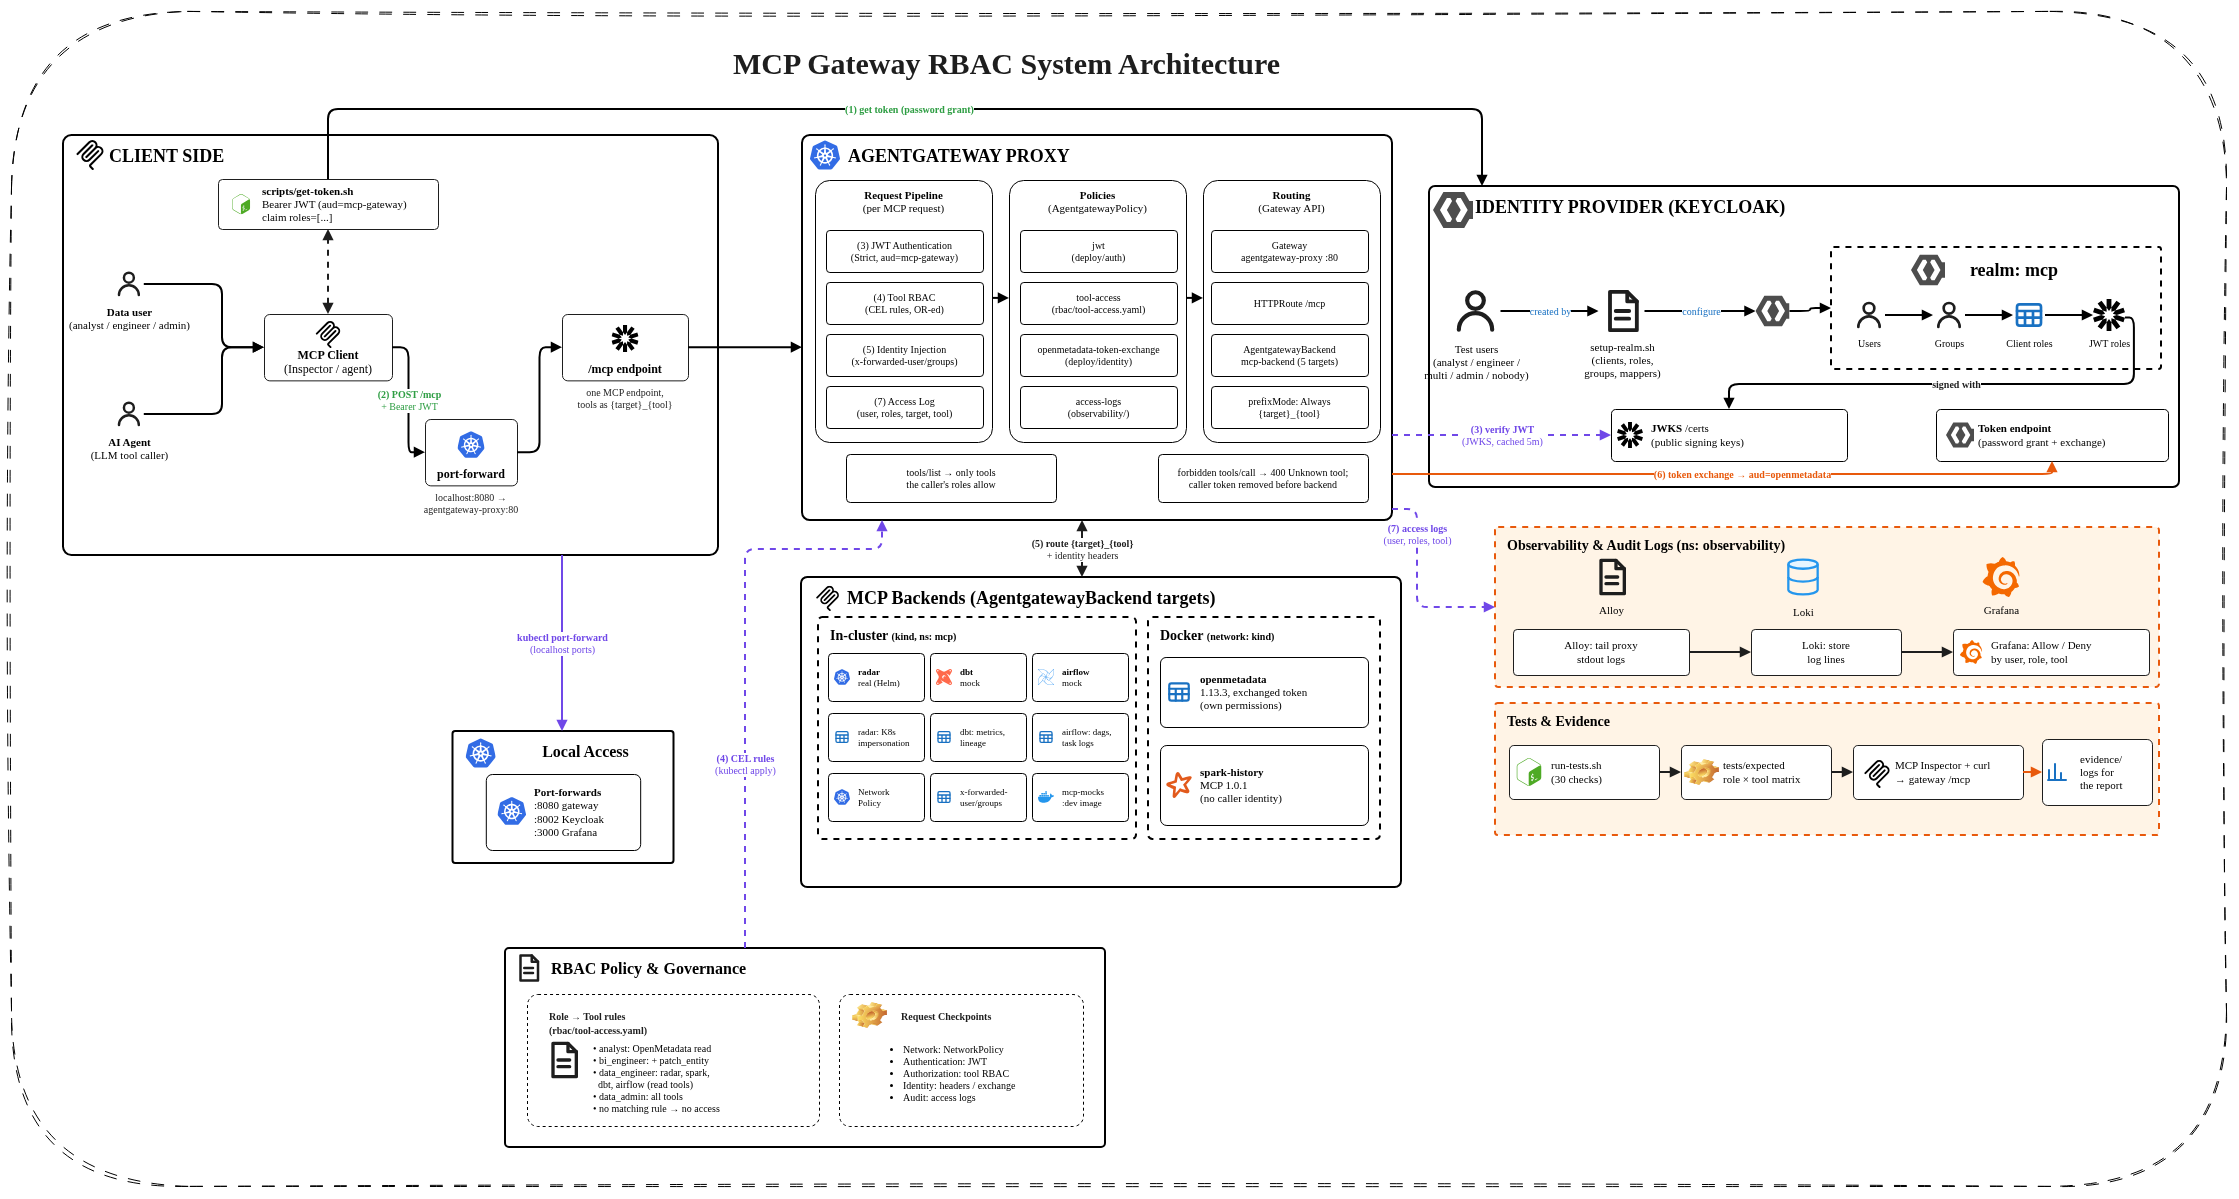
\includegraphics[width=1\textwidth]{system-architecture.png}
\caption{Kiến trúc tổng thể hệ thống}\label{fig:arch}\end{figure}

Hình~\ref{fig:docker} cho thấy mỗi thành phần thực sự chạy ở đâu. Hệ thống nằm trong ba vùng Docker nối với nhau qua network \texttt{kind}: toàn bộ cụm Kubernetes trong một container là node của kind, còn OpenMetadata và Spark History là hai nhóm container docker compose riêng. Vì vậy quy tắc mạng ở mục~\ref{sec:netpol} chỉ có hiệu lực trong vùng thứ nhất, và S4 mới đạt một phần. OpenMetadata gọi ngược vào Keycloak qua NodePort 30802 theo tên node \texttt{gatewayapi-control-plane}, nên tên cụm bị cố định. Trong các cổng ở Bảng~\ref{tab:ports}, chỉ cổng 8080 của gateway là cần cho nghiệp vụ; các cổng còn lại phục vụ quản trị và gỡ lỗi, và ở môi trường thật nên giữ ở mức nội bộ.

\begin{figure}[htbp]\centering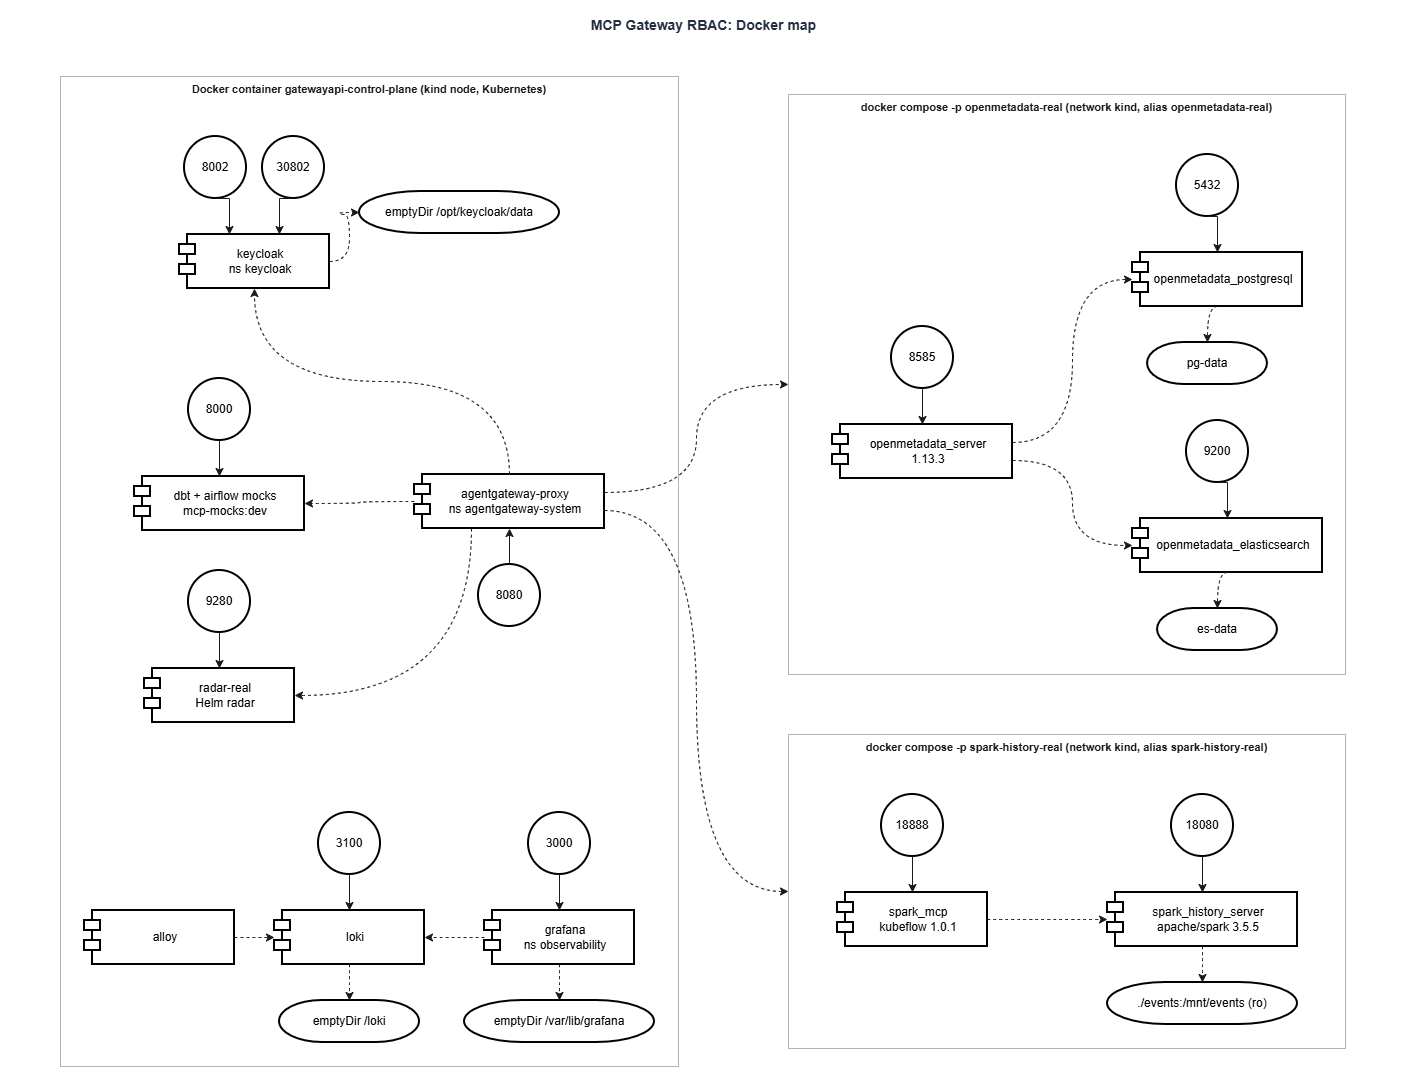
\includegraphics[width=0.72\textwidth]{docker-map.png}
\caption{Sơ đồ triển khai trên Docker: vùng chạy, cổng và volume}\label{fig:docker}\end{figure}

\begin{table}[H]\centering\caption{Cổng của các thành phần}\label{tab:ports}
{\singlespacing\renewcommand{\arraystretch}{1.15}\small
\begin{tabularx}{\textwidth}{|p{3.8cm}|c|X|}\hline
\textbf{Thành phần} & \textbf{Cổng} & \textbf{Ai dùng} \\ \hline
agentgateway & 8080 & AI Agent, người dùng (cổng duy nhất cần cho nghiệp vụ) \\ \hline
Keycloak & 8002 & Agent xin token; quản trị viên \\ \hline
Keycloak (NodePort) & 30802 & OpenMetadata kiểm tra token \\ \hline
Grafana & 3000 & Người vận hành xem dashboard \\ \hline
OpenMetadata & 8585 & Gateway; quản trị viên \\ \hline
Mock, radar & 8000, 9280 & Chỉ gateway, trong cụm \\ \hline
Spark MCP & 18888 & Chỉ gateway, qua network \texttt{kind} \\ \hline
Loki, PostgreSQL, Elasticsearch & 3100, 5432, 9200 & Chỉ nội bộ \\ \hline
\end{tabularx}}\end{table}

Keycloak, Loki và Grafana dùng \texttt{emptyDir} nên mất dữ liệu khi xóa cụm, còn OpenMetadata dùng volume có tên nên giữ lại. Sau mỗi lần dựng lại cụm, Keycloak có khóa ký mới trong khi OpenMetadata giữ cấu hình cũ, nên bước cấu hình OpenMetadata luôn được chạy lại. Script dọn dẹp chỉ xóa cụm kind và để nguyên hai nhóm container compose; hạn chế này được ghi nhận ở Chương 5.

% =====================================================================
\subsection{Luồng xử lý một yêu cầu}

Hình~\ref{fig:seq} mô tả một lệnh gọi công cụ; các số (1) đến (7) khớp với nhãn trên sơ đồ kiến trúc. Ở bước (1), agent dùng client ID và client secret xin token từ Keycloak; token cho biết token dành cho ai (\texttt{aud = mcp-gateway}), ai đang cầm (\texttt{azp}) và có vai trò gì (\texttt{roles}). Ở bước (2), agent gửi yêu cầu tới \texttt{/mcp} kèm token.

\begin{figure}[htbp]\centering
\begin{tikzpicture}[font=\small,yscale=0.68,
  tac/.style={draw,fill=gray!10,minimum width=2.3cm,minimum height=8mm,align=center},
  tn/.style={mui},tl/.style={mui,dashed}]
\foreach \x/\n/\t in {0/c/{AI Agent},3.3/k/Keycloak,6.6/g/agentgateway,9.9/b/{MCP backend},13.2/o/{Loki /\\ Grafana}}
  {\node[tac] (\n) at (\x,0) {\t}; \draw[gray] (\n.south) -- ++(0,-12.2);}
\newcommand{\msg}[5]{\draw[#5] (#1,#3) -- node[above,nhan]{#4} (#2,#3);}
\msg{0}{3.3}{-1.2}{(1) xin token}{tn}
\msg{3.3}{0}{-2.0}{JWT: aud, azp, roles}{tl}
\msg{0}{6.6}{-2.8}{(2) POST /mcp + Bearer token}{tn}
\draw[mui] (6.6,-3.4) -- ++(0.6,0) |- node[right,nhan,pos=0.25]{(3) xác thực JWT\\(JWKS, cache 5 phút)} (6.65,-4.4);
\draw[mui] (6.6,-4.9) -- ++(0.6,0) |- node[right,nhan,pos=0.25]{(4) RBAC theo tool\\(CEL, deny-by-default)} (6.65,-5.9);
\draw[mui] (6.6,-6.4) -- ++(0.6,0) |- node[right,nhan,pos=0.25]{(5) đặt header định danh,\\xóa token gốc} (6.65,-7.4);
\msg{6.6}{9.9}{-8.3}{tools/call (không có token)}{tn}
\msg{9.9}{6.6}{-9.1}{kết quả}{tl}
\msg{6.6}{0}{-9.9}{kết quả / lỗi ``Unknown tool''}{tl}
\msg{6.6}{13.2}{-10.9}{(7) access log: user, roles, tool, status}{tn}
\node[nhan,fill=white,draw,dashed] at (8.25,-11.7) {(6) riêng OpenMetadata: token exchange trước bước gửi};
\end{tikzpicture}
\caption{Sơ đồ tuần tự của một lệnh gọi công cụ}\label{fig:seq}\end{figure}

Bước (3) đến (5) diễn ra trong gateway theo thứ tự bắt buộc: kiểm tra chữ ký token bằng khóa công khai của Keycloak, kiểm tra vai trò có được dùng công cụ không, và chỉ khi cả hai đạt mới ghi danh tính vào header, xóa token gốc và chuyển yêu cầu tới backend. Nếu header được ghi trước khi kiểm tra token, kẻ tấn công có thể tự điền danh tính giả; nếu token bị xóa trước bước (6), OpenMetadata không đổi được token. Bước (6) chỉ áp dụng cho OpenMetadata: gateway đổi token gốc lấy token mới chỉ dùng được cho hệ thống này, để nó tự áp quyền theo đúng người gọi. Bước (7) ghi mọi yêu cầu vào access log.

Hình~\ref{fig:decision} bổ sung các nhánh bị từ chối. Token không hợp lệ trả về HTTP 401; không có quyền dùng công cụ trả về HTTP 400 kèm \texttt{Unknown tool}, tức công cụ bị coi như không tồn tại. Cách này không để lộ công cụ nào có thật, nhưng làm lỗi phân quyền trông giống lỗi gõ sai tên, vấn đề được xử lý ở mục~\ref{sec:obs}.

\begin{figure}[htbp]\centering
\begin{tikzpicture}[node distance=3.5mm and 10mm]
\node[khoi] (req) {Yêu cầu tới \texttt{/mcp}};
\node[quyetdinh,below=of req] (tok) {Token hợp lệ?};
\node[khoi,right=of tok,fill=red!8] (e401) {HTTP 401};
\node[quyetdinh,below=of tok] (m) {Phương thức?};
\node[khoi,right=of m,xshift=4mm] (list) {Trả danh mục\\đã lọc theo quyền};
\node[quyetdinh,below=of m] (rule) {Có quy tắc\\cho phép?};
\node[khoi,right=of rule,fill=red!8] (e400) {HTTP 400\\``Unknown tool''};
\node[khoi,below=of rule] (hdr) {Đặt header định danh,\\xóa token gốc};
\node[khoi,below=of hdr,fill=green!8] (be) {Chuyển tới backend\\HTTP 200};
\node[khoi,left=18mm of rule] (log) {Ghi access log\\(mọi nhánh)};
\draw[mui] (req) -- (tok);
\draw[mui] (tok) -- node[above,nhan]{không} (e401);
\draw[mui] (tok) -- node[left,nhan]{có} (m);
\draw[mui] (m) -- node[above,nhan]{tools/list} (list);
\draw[mui] (m) -- node[left,nhan]{tools/call} (rule);
\draw[mui] (rule) -- node[above,nhan]{không} (e400);
\draw[mui] (rule) -- node[left,nhan]{có} (hdr);
\draw[mui] (hdr) -- (be);
\draw[dashed,gray,thick] (log.north) |- (tok.west); \draw[dashed,gray,thick] (log.east) -- (rule.west); \draw[dashed,gray,thick] (log.south) |- (be.west);
\end{tikzpicture}
\caption{Lưu đồ quyết định của gateway}\label{fig:decision}\end{figure}

% =====================================================================
\subsection{Các thành phần nền tảng của gateway}\label{sec:netpol}

Mọi yêu cầu tới \texttt{/mcp} được chuyển tới một backend của agentgateway chứa năm target; gateway gộp danh mục của cả năm và thêm tên target vào trước tên công cụ, ví dụ \texttt{radar\_list\_namespaces} (F1, F2). Ràng buộc đi kèm là tên target phải giống hệt nhau ở tên mock, Service, quy tắc phân quyền và bộ kiểm thử; lệch một ký tự là công cụ bị chặn mà không có lỗi nào chỉ ra nguyên nhân. Cấu hình được trích ở Phụ lục B.

Quy tắc xác thực gắn vào Gateway thay vì từng route, nên route thêm sau cũng được bảo vệ. Khóa công khai của Keycloak được lưu đệm năm phút, nên khi Keycloak đổi khóa, gateway có thể từ chối token mới trong tối đa năm phút. Sau khi token hợp lệ, gateway \emph{ghi đè} ba header \texttt{x-forwarded-user}, \texttt{x-forwarded-groups} và \texttt{x-agent-id} bằng giá trị lấy từ token, nên header giả do client gửi bị thay thế. Token gốc được giữ tạm trong một header nội bộ cho việc đổi token của OpenMetadata, rồi bị một quy tắc thứ hai xóa trước khi rời gateway (S3); thiếu quy tắc thứ hai thì mọi backend đều nhận được token gốc.

Toàn bộ phân quyền nằm trong một chính sách duy nhất, mỗi quy tắc là một biểu thức CEL kiểm tra vai trò, target và tên công cụ; các quy tắc được nối bằng phép HOẶC nên người có nhiều vai trò nhận hợp quyền (S2). Nhóm chọn một chính sách duy nhất sau khi thử nghiệm cho thấy cách gateway kết hợp nhiều chính sách khó đoán. Chính sách hiện chứa bốn vai trò cho người dùng và mười vai trò cho AI Agent (mục~\ref{sec:agent}).

Một NetworkPolicy chỉ cho lưu lượng vào namespace backend nếu đến từ namespace của gateway. Đây là mắt xích giữ cho danh tính có giá trị: backend tin header \texttt{x-forwarded-user} vì chỉ gateway gửi được nó, nên nếu một pod khác gọi thẳng được backend thì pod đó có thể tự đặt header này. Hai backend thật chạy bằng Docker nằm ngoài cụm nên không được quy tắc này bảo vệ.

% =====================================================================
\subsection{Mock MCP server và danh mục công cụ}

Kiểm thử phân quyền đòi hỏi gọi từng công cụ với từng vai trò, kể cả công cụ có tác động, điều vừa rủi ro vừa không lặp lại được trên hệ thống thật (mục~\ref{sec:ch3-mock}). Năm mock viết bằng Python với FastMCP, dùng chung một module (Phụ lục C) gồm hai hàm: hàm tạo server ở chế độ không lưu phiên để bất kỳ bản sao nào của gateway cũng phục vụ được, và hàm ghi lại ``ai đang gọi'' ở đầu mỗi công cụ. Hàm thứ hai ghi target, công cụ, tham số, ba header danh tính, có header \texttt{Authorization} hay không, và nếu có token thì chỉ lấy vài claim không nhạy cảm, không bao giờ ghi bản thân token. Kết quả được trả về trong trường \texttt{seen\_by\_mock}, nhờ đó bộ kiểm thử kiểm tra trực tiếp từ phía backend rằng token gốc đã bị xóa (S3) và danh tính đúng người gọi. Cả năm mock dùng chung một image, chạy thành năm Deployment có Service đặt tên đúng bằng tên target.

Mỗi mock mô phỏng các công cụ tiêu biểu với tên và tham số theo MCP server chính thức của phần mềm gốc, để khi chuyển sang phần mềm thật thì quy tắc phân quyền không phải sửa. Danh mục gồm 21 công cụ (Bảng~\ref{tab:tools}; mô tả chi tiết ở Phụ lục C), trong đó 15 công cụ đọc và 6 công cụ ghi hoặc thực thi. Việc tách đọc và ghi là nền tảng của thiết kế vai trò ở mục sau.

\begin{table}[H]\centering\caption{Danh mục 21 công cụ theo target và loại}\label{tab:tools}
{\singlespacing\renewcommand{\arraystretch}{1.15}\small
\begin{tabularx}{\textwidth}{|p{2.3cm}|X|p{3.6cm}|}\hline
\textbf{Target} & \textbf{Công cụ đọc} & \textbf{Công cụ ghi / thực thi} \\ \hline
radar & list\_namespaces, list\_resources, get\_pod\_logs & manage\_workload \\ \hline
spark-history & list\_applications, get\_stage, get\_job\_bottlenecks & -- \\ \hline
openmetadata & search\_metadata, get\_entity\_details, get\_entity\_lineage & patch\_entity \\ \hline
dbt & list\_metrics, query\_metrics, get\_model\_health, get\_lineage & test \\ \hline
airflow & list\_dags, get\_dag\_run, get\_task\_logs & trigger\_dag, pause\_dag \\ \hline
\textbf{Tổng} & \textbf{15} & \textbf{6} \\ \hline
\end{tabularx}}\end{table}

% =====================================================================
\subsection{Thiết lập danh tính AI Agent trên Keycloak}\label{sec:agent}

Người dùng đăng nhập bằng mật khẩu và nhận vai trò theo chức danh (\texttt{analyst}, \texttt{bi\_engineer}, \texttt{data\_engineer}, \texttt{data\_admin}); AI Agent không có người đăng nhập nên mỗi agent là một client riêng trên Keycloak, tự xin token bằng luồng client credentials. Cả hai loại được đặt trong cùng một realm và nhận vai trò từ cùng client \texttt{mcp-gateway}, nên token có cùng cấu trúc và gateway dùng một bộ quy tắc cho cả hai; tách hai realm sẽ buộc gateway tin hai nơi cấp token và viết mọi quy tắc hai lần. Client và vai trò của agent được khai báo trong một file cấu hình và nạp bằng tính năng nhập một phần (partial import) của Keycloak (Phụ lục D), giữ nguyên phần realm dành cho người dùng.

Vai trò của agent được chia theo năng lực trên từng hệ thống thay vì theo chức danh, mỗi hệ thống có mức \textit{viewer} chỉ đọc và mức \textit{operator} hoặc \textit{editor} có thêm thao tác ghi. Nhờ vậy agent xử lý sự cố, cần khởi động lại ứng dụng trên Kubernetes và đọc thông tin Spark, chỉ cần ghép \texttt{kube\_operator} với \texttt{spark\_viewer} thay vì nhận vai trò \texttt{data\_engineer} kèm nhiều quyền thừa. Bảng~\ref{tab:agents} liệt kê mười agent, trong đó \texttt{no-access} không có vai trò để chứng minh mặc định từ chối, và \texttt{platform-admin} có toàn quyền để chứng minh đủ 21 công cụ đều gọi được, không dùng cho công việc thường ngày. Ma trận được lưu thành file JSON làm kết quả mong đợi cho bộ kiểm thử ở Chương 5.

\begin{table}[H]\centering\caption{Ma trận Agent -- Vai trò -- số công cụ được phép}\label{tab:agents}
{\singlespacing\renewcommand{\arraystretch}{1.15}\small
\begin{tabularx}{\textwidth}{|p{4.6cm}|X|c|}\hline
\textbf{Agent} & \textbf{Vai trò} & \textbf{Số công cụ} \\ \hline
cluster-observer & kube\_viewer & 3 \\ \hline
incident-response & kube\_operator, spark\_viewer & 7 \\ \hline
spark-diagnostic & spark\_viewer & 3 \\ \hline
metadata-discovery & metadata\_viewer & 3 \\ \hline
metadata-steward & metadata\_editor & 4 \\ \hline
dbt-quality & dbt\_operator & 5 \\ \hline
airflow-monitor & airflow\_viewer & 3 \\ \hline
airflow-operator & airflow\_operator & 5 \\ \hline
platform-admin & platform\_admin (khẩn cấp) & 21 \\ \hline
no-access & (không có) & 0 \\ \hline
\end{tabularx}}\end{table}

Mỗi agent có secret riêng để có thể thu hồi từng agent mà không ảnh hưởng các agent khác. Secret được sinh ngẫu nhiên dài 256 bit, ghi thẳng vào Kubernetes Secret, không in ra màn hình và không lưu vào kho mã. Bước sinh secret giữ nguyên secret đã có, và dừng lại nếu chỉ một phần secret tồn tại, vì sinh lại một phần sẽ làm Kubernetes và Keycloak giữ hai giá trị khác nhau và agent không xin được token. Khi nạp client, giá trị giữ chỗ trong file cấu hình được thay bằng secret đọc từ Kubernetes ngay lúc chạy.

% =====================================================================
\subsection{Ma trận phân quyền theo vai trò}\label{sec:rolematrix}

Bảng~\ref{tab:rolematrix} tổng hợp quyền của từng vai trò trên năm hệ thống, gồm vai trò của người dùng, vai trò năng lực của agent và các tổ hợp nhiều vai trò. ``Đọc'' là toàn bộ công cụ đọc của hệ thống đó, ``Đọc + ghi'' là thêm công cụ ghi hoặc thực thi (Bảng~\ref{tab:tools}), cột ``Tổng'' là số công cụ được phép. Mọi quyền trong bảng đều được khai báo trong một chính sách Allow duy nhất; công cụ không có quy tắc nào khớp thì bị ẩn khỏi danh mục và bị từ chối khi gọi.

\begin{table}[H]\centering\caption{Ma trận Vai trò -- Hệ thống -- Công cụ được phép}\label{tab:rolematrix}
{\singlespacing\renewcommand{\arraystretch}{1.15}\setlength{\tabcolsep}{4pt}\small
\begin{tabularx}{\textwidth}{|>{\raggedright\arraybackslash}p{3.3cm}|*{5}{>{\centering\arraybackslash}X|}c|}\hline
\textbf{Vai trò} & \textbf{radar} & \textbf{spark-history} & \textbf{open-\allowbreak metadata} & \textbf{dbt} & \textbf{airflow} & \textbf{Tổng} \\ \hline
\multicolumn{7}{|l|}{\textit{Vai trò người dùng (theo chức danh)}} \\ \hline
analyst & -- & -- & Đọc & -- & -- & 3 \\ \hline
bi\_engineer & -- & -- & Đọc + ghi & -- & -- & 4 \\ \hline
data\_engineer & Đọc & Đọc & Đọc & Đọc & Đọc & 16 \\ \hline
data\_engineer + bi\_engineer & Đọc & Đọc & Đọc + ghi & Đọc & Đọc & 17 \\ \hline
data\_admin & Tất cả & Tất cả & Tất cả & Tất cả & Tất cả & 21 \\ \hline
(không có vai trò) & -- & -- & -- & -- & -- & 0 \\ \hline
\multicolumn{7}{|l|}{\textit{Vai trò của AI Agent (theo năng lực)}} \\ \hline
kube\_viewer & Đọc & -- & -- & -- & -- & 3 \\ \hline
kube\_operator & Đọc + ghi & -- & -- & -- & -- & 4 \\ \hline
spark\_viewer & -- & Đọc & -- & -- & -- & 3 \\ \hline
metadata\_viewer & -- & -- & Đọc & -- & -- & 3 \\ \hline
metadata\_editor & -- & -- & Đọc + ghi & -- & -- & 4 \\ \hline
dbt\_viewer & -- & -- & -- & Đọc & -- & 4 \\ \hline
dbt\_operator & -- & -- & -- & Đọc + ghi & -- & 5 \\ \hline
airflow\_viewer & -- & -- & -- & -- & Đọc & 3 \\ \hline
airflow\_operator & -- & -- & -- & -- & Đọc + ghi & 5 \\ \hline
kube\_operator + spark\_viewer & Đọc + ghi & Đọc & -- & -- & -- & 7 \\ \hline
platform\_admin (khẩn cấp) & Tất cả & Tất cả & Tất cả & Tất cả & Tất cả & 21 \\ \hline
\end{tabularx}}\end{table}

Ma trận dựa trên ba nguyên tắc. Thứ nhất là quyền tối thiểu: mỗi vai trò chỉ nhận công cụ cần cho công việc của mình. Thứ hai là tách đọc và ghi: công cụ ghi hoặc thực thi làm thay đổi trạng thái hệ thống (khởi động lại workload, sửa metadata, chạy kiểm thử dbt, kích hoạt hoặc tạm dừng DAG) nên chỉ cấp cho vai trò cần đúng thao tác đó, không đi kèm theo quyền đọc. Thứ ba là cộng quyền: các quy tắc được kết hợp bằng phép OR, nên người dùng hoặc agent có nhiều vai trò nhận hợp các quyền mà không cần quy tắc riêng cho từng tổ hợp.

Với người dùng, \texttt{analyst} chỉ cần tìm và hiểu dữ liệu nên nhận ba công cụ đọc của OpenMetadata (tìm kiếm, xem chi tiết, xem lineage), không được sửa metadata và không chạm vào hạ tầng, vì log và tình trạng pipeline không thuộc công việc phân tích và có thể chứa dữ liệu nội bộ. \texttt{bi\_engineer} xây báo cáo trên các bảng dữ liệu và chịu trách nhiệm mô tả, gắn thẻ cho chúng, nên được thêm \texttt{patch\_entity}. \texttt{data\_engineer} vận hành pipeline và phải chẩn đoán sự cố xuyên suốt năm hệ thống (log pod, điểm nghẽn Spark, lineage, tình trạng model dbt, log task Airflow), nên được đọc ở cả năm; ngược lại cả sáu công cụ ghi đều bị giữ lại vì chúng tác động lên hệ thống đang chạy, phải đi qua \texttt{data\_admin} hoặc agent vận hành chuyên trách. \texttt{data\_admin} không bị giới hạn theo target, nên một backend thêm vào sau cũng tự động thuộc quyền quản trị; vai trò này chỉ dành cho số ít người và mọi lệnh gọi vẫn được ghi log. Token hợp lệ nhưng không có vai trò không nhận công cụ nào, cho thấy xác thực thành công không đồng nghĩa với được phân quyền.

Tổ hợp \texttt{data\_engineer} + \texttt{bi\_engineer} (người dùng \texttt{multi.user}) nhận 17 công cụ, đúng bằng 16 công cụ của \texttt{data\_engineer} cộng \texttt{patch\_entity} của \texttt{bi\_engineer}. Đây là lý do nhóm không dùng quy tắc Deny để giới hạn theo vai trò: thí nghiệm chồng lấn chính sách cho thấy Deny được xét theo người dùng chứ không theo vai trò và luôn thắng Allow, nên nếu chặn radar với \texttt{bi\_engineer} thì người dùng giữ cả hai vai trò cũng mất radar dù \texttt{data\_engineer} cho phép. Deny chỉ phù hợp với lệnh cấm tuyệt đối áp dụng cho mọi vai trò.

Với agent, vai trò được chia theo năng lực trên từng hệ thống (mục~\ref{sec:agent}). Mức \textit{operator} hoặc \textit{editor} bao gồm luôn quyền đọc của mức \textit{viewer}, vì agent cần đọc trạng thái trước khi hành động. Spark History chỉ có mức \textit{viewer} vì danh mục hiện tại không có công cụ ghi cho hệ thống này. Tổ hợp \texttt{kube\_operator} + \texttt{spark\_viewer} của agent xử lý sự cố cho 7 công cụ, ít hơn nhiều so với 16 công cụ nếu cấp \texttt{data\_engineer}. \texttt{platform\_admin} có toàn quyền như \texttt{data\_admin} nhưng chỉ dùng khi khẩn cấp và để kiểm chứng đủ 21 công cụ, không gán cho agent làm việc thường ngày.

% =====================================================================
\subsection{Tự động hóa triển khai}\label{sec:auto}

Việc dựng môi trường chia làm hai giai đoạn theo tần suất. Giai đoạn khởi tạo chạy một lần: tạo cụm kind, cài Calico, Gateway API, agentgateway và đóng gói image mock; các bước này chậm, tải nhiều image và hiếm khi thay đổi. Giai đoạn khởi động chạy mỗi khi bắt đầu làm việc, do script up đảm nhiệm, và chỉ áp lại cấu hình nên nhanh.

Script up gồm ba tầng (Hình~\ref{fig:up}, Phụ lục E). Tầng ngoài là một lớp bọc PowerShell cho người dùng Windows: nó chỉ đổi thư mục mã nguồn sang đường dẫn WSL, giao việc cho hai script bash và đo tổng thời gian, để logic dựng hệ thống chỉ tồn tại ở một nơi. Tầng giữa là script áp cấu hình, áp các lớp cấu hình theo thứ tự phụ thuộc không đảo được: Keycloak phải chạy xong mới tạo được realm, realm phải có mới tạo được client cho agent và lấy được secret của gateway, secret này phải có thì việc đổi token cho OpenMetadata mới hoạt động, và chỉ sau đó mới áp phân quyền, NetworkPolicy và access log. Tầng cuối là script giám sát, cài Loki, Alloy, Grafana và chờ cả ba sẵn sàng.

\begin{figure}[htbp]\centering
\begin{tikzpicture}[node distance=3mm,every node/.style={font=\small}]
\node[khoi,fill=gray!10,text width=9cm] (w) {Lớp bọc PowerShell: tìm thư mục mã nguồn, chuyển sang WSL, bấm giờ};
\node[khoi,below=of w,text width=9cm] (a) {Script áp cấu hình\\gateway, mock, route $\rightarrow$ Keycloak + realm (nếu chưa có)\\$\rightarrow$ client AI Agent và secret $\rightarrow$ xác thực JWT, token exchange\\$\rightarrow$ phân quyền theo công cụ $\rightarrow$ NetworkPolicy $\rightarrow$ access log};
\node[khoi,below=of a,text width=9cm] (g) {Script giám sát: Loki, Alloy, Grafana + dashboard};
\node[quyetdinh,below=of g] (ok) {Mã thoát = 0?};
\node[khoi,right=10mm of ok,fill=red!8] (x) {Dừng, báo lỗi\\và thời gian đã chạy};
\node[khoi,left=10mm of ok,fill=green!8] (e) {Báo sẵn sàng\\và tổng thời gian};
\draw[mui] (w)--(a); \draw[mui] (a)--(g); \draw[mui] (g)--(ok);
\draw[mui] (ok)--node[above,nhan]{không}(x); \draw[mui] (ok)--node[above,nhan]{có}(e);
\end{tikzpicture}
\caption{Cấu trúc và luồng của script khởi động}\label{fig:up}\end{figure}

Script được thiết kế idempotent vì trong thực tế nó hay bị dừng giữa chừng và cách khắc phục đơn giản nhất là chạy lại. Cấu hình Kubernetes được áp theo kiểu khai báo nên áp lại không tạo bản sao; realm chỉ được tạo khi chưa có, vì tạo lại sẽ sinh khóa mới và làm mọi token đang dùng mất hiệu lực; secret của agent cũng chỉ được sinh khi chưa có. Các script bash chạy với \texttt{set -euo pipefail} và mọi bước chờ đều có giới hạn thời gian, nên script không báo thành công khi một bước thất bại và không treo khi một thành phần không lên; tầng PowerShell kiểm tra mã thoát của WSL và báo lại kèm thời gian đã chạy. Script down chỉ xóa toàn bộ cụm.

% =====================================================================
\subsection{Giám sát allow/deny}\label{sec:obs}

Access log mặc định của agentgateway chỉ ghi phương thức, đường dẫn và mã trạng thái, nên biết có bao nhiêu yêu cầu bị chặn nhưng không biết ai bị chặn ở công cụ nào. Một quy tắc access log được gắn vào Gateway để ghi thêm sáu trường: tên người dùng, mã agent, danh sách vai trò, phương thức MCP, target và tên công cụ (Phụ lục F). Các trường được lấy từ token đã kiểm tra chứ không từ header do client gửi, để không ai ghi được tên người khác vào log; yêu cầu không có token được ghi là \texttt{anonymous}, và token không bao giờ được ghi.

Alloy chỉ thu log của các pod \texttt{agentgateway-proxy} và gửi về Loki; Grafana đọc từ Loki và tự nạp dashboard khi khởi động (Hình~\ref{fig:obs}). Bộ ba này đủ nhẹ cho máy cá nhân (mục~\ref{sec:ch3-obs}) và không đòi hỏi sửa gateway, nên có thể thêm hoặc gỡ mà không ảnh hưởng luồng xử lý chính.

\begin{figure}[htbp]\centering
\begin{tikzpicture}[node distance=9mm]
\node[khoi] (gw) {agentgateway\\stdout};
\node[khoi,right=of gw] (al) {Alloy\\thu log pod gateway};
\node[khoi,right=of al] (lk) {Loki\\lưu, đánh nhãn};
\node[khoi,right=of lk] (gr) {Grafana\\dashboard};
\node[khoi,below=6mm of al,fill=gray!8,text width=3.4cm] (pol) {Chính sách access log:\\user, agent\_id, roles,\\target, tool};
\node[khoi,below=6mm of gr,fill=gray!8,text width=3.6cm] (q) {LogQL: 200 → allow\\400 + Unknown tool → deny};
\draw[mui] (gw)--(al); \draw[mui] (al)--(lk); \draw[mui] (lk)--(gr);
\draw[mui,dashed] (pol.west) -| (gw.south); \draw[mui,dashed] (q)--(gr);
\end{tikzpicture}
\caption{Đường ống dữ liệu quan sát allow/deny}\label{fig:obs}\end{figure}

Vì gateway không có mã lỗi riêng cho ``không có quyền'' (Hình~\ref{fig:decision}), dashboard tự phân loại: lệnh gọi công cụ trả HTTP 200 là cho phép, trả HTTP 400 kèm \texttt{Unknown tool} là bị chặn. Quy tắc này không phân biệt được thiếu quyền với gõ sai tên công cụ, dù trường hợp sau hiếm vì agent lấy tên từ danh mục, và phụ thuộc thông báo lỗi của agentgateway 1.5.0 nên cần kiểm tra lại khi nâng cấp. Dashboard có tám ô xếp từ tổng quan xuống chi tiết (Hình~\ref{fig:dashboard}): hai ô số liệu tổng số lệnh cho phép và bị chặn; bốn biểu đồ theo thời gian, người dùng, vai trò và công cụ để khoanh vùng; hai ô log hiển thị từng lệnh gọi, trong đó một ô chỉ chứa lệnh bị chặn. Người vận hành nhờ đó trả lời được ``ai đã gọi gì và có bị chặn không'' bằng vài thao tác lọc (O2, S5).

\begin{figure}[htbp]\centering
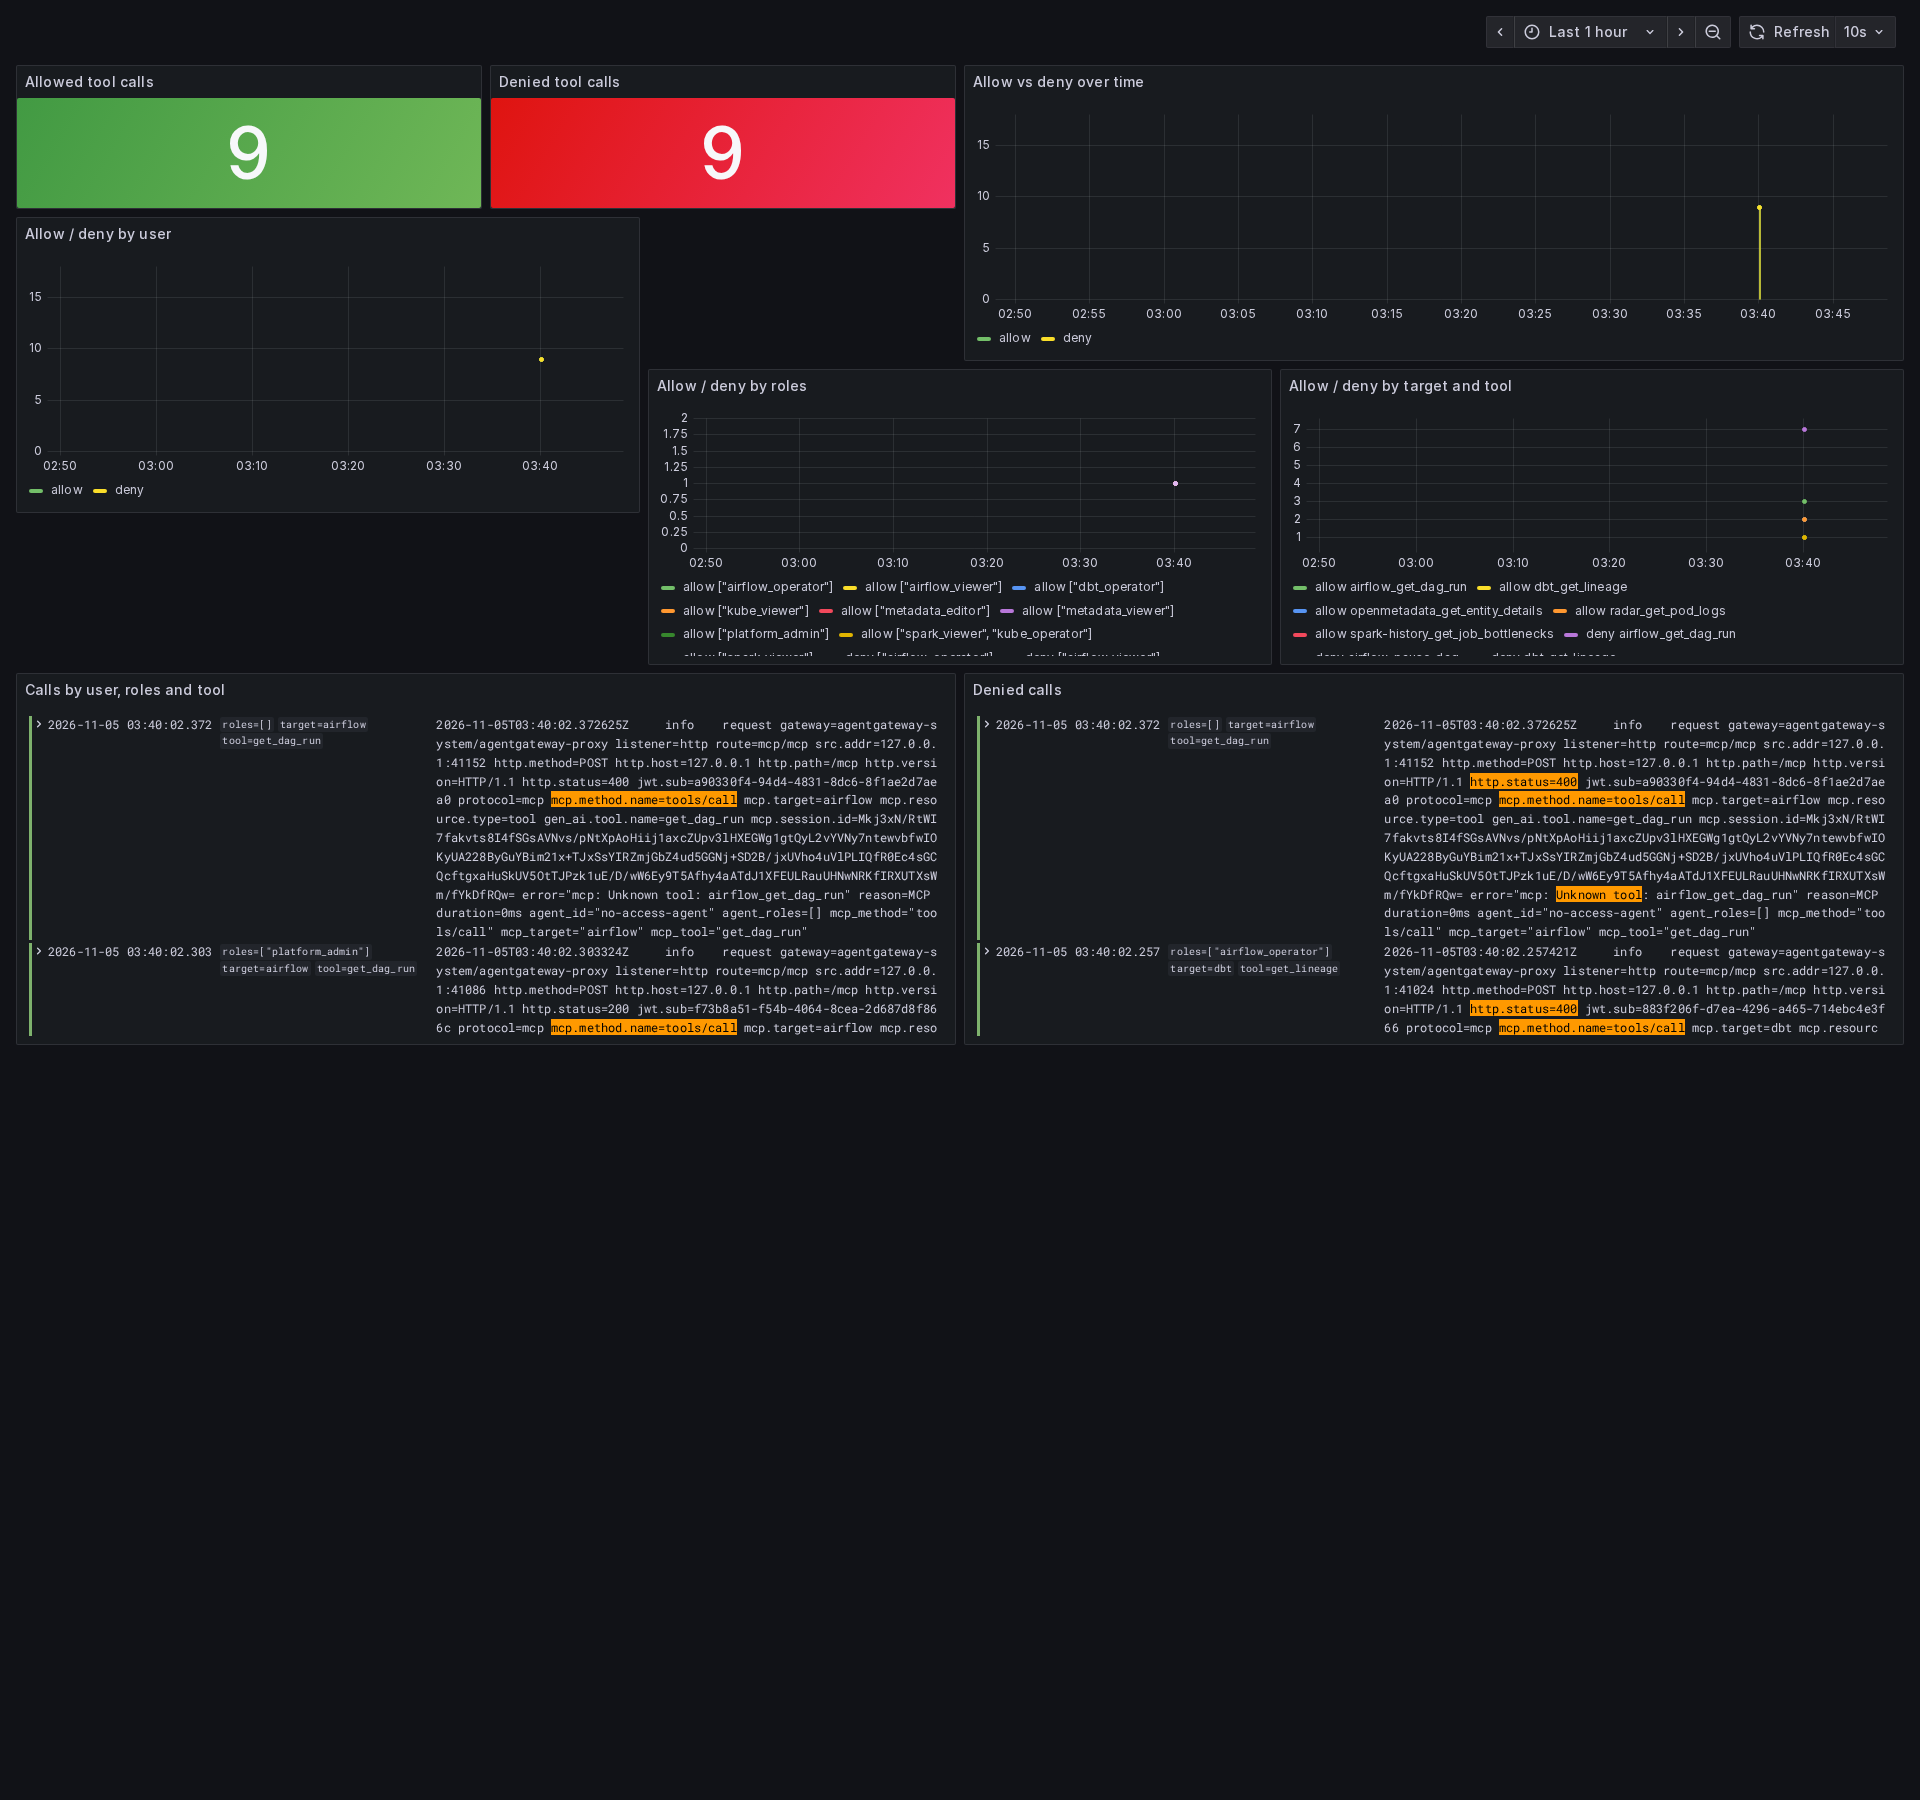
\includegraphics[width=0.8\textwidth,trim=0 750 0 0,clip]{grafana-allow-deny.png}
\caption{Dashboard giám sát allow/deny trên Grafana}\label{fig:dashboard}\end{figure}
% ===== chapters/ch5-kiem-chung.tex =====
\chuong{KIỂM CHỨNG PROOF OF CONCEPT}
\begingroup\setlength{\emergencystretch}{2em}
\subsection{Kịch bản kiểm chứng}

Mỗi yêu cầu ở Bảng~\ref{tab:yeucau} được gắn với ít nhất một kịch bản, có tiêu chí đạt viết sẵn từ trước và đầu ra kiểm tra được (Bảng~\ref{tab:scenarios}). Các kịch bản chạy ở hai mức. Ở mức tĩnh, kịch bản K9 đối chiếu ma trận kỳ vọng với danh mục công cụ, chính sách phân quyền và cấu hình realm mà không cần đến cụm. Ở mức đầu cuối, hai bộ kiểm thử, một cho danh mục công cụ và một cho phân quyền theo agent, dùng MCP Python SDK 1.30.0 gọi thật vào \texttt{/mcp} và dừng ngay ở phép so sánh sai đầu tiên. Kết quả ``PASS'' vì thế chỉ xuất hiện khi mọi phép so đều đúng. Riêng thăm dò NetworkPolicy và đọc access log được làm thủ công, đầu ra lưu lại làm bằng chứng.

\begin{table}[H]\centering\caption{Kịch bản kiểm chứng theo yêu cầu}\label{tab:scenarios}
{\singlespacing\renewcommand{\arraystretch}{1.15}\small
\begin{tabularx}{\textwidth}{|c|>{\raggedright\arraybackslash}p{1.5cm}|>{\raggedright\arraybackslash}X|>{\raggedright\arraybackslash}p{4.2cm}|}\hline
\textbf{Mã} & \textbf{Yêu cầu} & \textbf{Kịch bản và tiêu chí đạt} & \textbf{Bằng chứng} \\ \hline
K1 & F1, F2 & Liệt kê và gọi cả 21 công cụ qua \texttt{/mcp}; danh sách tên đã sắp xếp phải trùng khớp và không lệnh nào lỗi & \path{gateway-smoke.txt} (08/10) \\ \hline
K2 & F3, S2 & Mười agent xin token; \texttt{tools/list} của mỗi agent phải trùng ma trận kỳ vọng & \path{agent-rbac-smoke.txt} (29/10) \\ \hline
K3 & S1 & Mỗi agent gọi một công cụ ngoài quyền và phải bị từ chối; ẩn tạm một công cụ rồi gọi thẳng tên của nó & \path{agent-rbac-smoke.txt}, \path{tool-denial*.txt} \\ \hline
K4 & S2, S3 & Token mang đúng \texttt{aud}, \texttt{azp}, \texttt{roles}; backend báo lại đúng header danh tính & \path{agent-rbac-smoke.txt} \\ \hline
K5 & S1, S3 & Gọi bằng curl khi thiếu token, khi gửi header danh tính giả, và kiểm tra token gốc không tới backend & Chưa lưu đầu ra \\ \hline
K6 & S4 & Thăm dò backend radar từ namespace \texttt{default} và từ namespace của gateway & \path{agent-rbac-smoke.txt} \\ \hline
K7 & S5, O2 & Mọi lệnh cho phép và bị chặn phải có bản ghi kèm danh tính agent trong access log và trên dashboard & Access log, ảnh dashboard \\ \hline
K8 & O1 & Năm lần \textit{warm start} liên tiếp, mỗi lần kèm kiểm thử phân quyền & \path{benchmarks/warm.md} \\ \hline
K9 & F2, S2 & Kiểm thử tĩnh đối chiếu ma trận, danh mục, chính sách và realm & \path{static_contract_test.mjs} \\ \hline
\end{tabularx}}\end{table}

Môi trường thử là cụm kind một node chạy Kubernetes v1.37.0 với Calico v3.33.0 trên WSL2, cùng agentgateway v1.5.0 và Keycloak 26.2.5. Bằng chứng được ghi trong ba đợt. Đợt ngày 08/10/2026 dành cho danh mục và thí nghiệm ẩn công cụ, đợt 29/10/2026 cho phân quyền theo agent, cô lập mạng và kiểm toán, còn đợt 05/11/2026 cho dashboard và thời gian khởi động. Các mục dưới đây trình bày kết quả lần lượt theo chức năng, phân quyền, an toàn rồi vận hành; Bảng~\ref{tab:ch5-goals} ở cuối chương gom lại theo từng yêu cầu.

\subsection{Kết quả chức năng}

Kịch bản K1 đạt trọn vẹn. Gateway trả về 21 công cụ, và cả 21 lệnh gọi đều thành công. Bộ kiểm thử so toàn bộ danh sách tên đã sắp xếp thay vì chỉ đếm, nên chỉ cần một công cụ thiếu, thừa hay sai tiền tố là lần chạy thất bại. Số công cụ theo target khớp Bảng~\ref{tab:tools}, với radar 4, spark-history 3, openmetadata 4, dbt 5 và airflow 5. Access log của cùng lượt chạy cho thấy gateway tách tên đầy đủ trở lại thành target và tên gốc, chẳng hạn \texttt{mcp.target=spark-history} đi cùng \texttt{gen\_ai.tool.name=get\_stage}. Đây cũng chính là hai trường mà quy tắc phân quyền đọc.

Có điều kiện đi kèm kết quả này. Lượt chạy ngày 08/10/2026 diễn ra trước khi bật xác thực JWT, nên access log ghi \texttt{user="anonymous"}. Sau khi bật JWT, danh mục đủ 21 công cụ được xác nhận lại qua \texttt{platform-admin-agent} ở kịch bản K2, nhưng agent này chỉ gọi một công cụ. F1 và F2 vì vậy có bằng chứng đầy đủ ở bước khám phá dưới JWT, trong khi bằng chứng gọi đủ 21 công cụ thuộc về cấu hình chưa bật JWT.

\subsection{Kết quả phân quyền}

Trong lượt chạy ngày 29/10/2026, cả mười agent đều đạt kịch bản K2. Bảng~\ref{tab:rbac} đặt số kỳ vọng, tính từ ma trận agent, vai trò và công cụ, cạnh số thực tế. Bộ kiểm thử so khớp từng tên chứ không so số lượng, nên việc hai cột trùng nhau có nghĩa là cả 210 ô của ma trận (10 agent nhân 21 công cụ) đều đúng ở bước khám phá.

\begin{table}[H]\centering\caption{Kết quả kiểm thử phân quyền theo agent}\label{tab:rbac}
{\singlespacing\renewcommand{\arraystretch}{1.15}\small
\begin{tabularx}{\textwidth}{|p{3.6cm}|X|>{\centering\arraybackslash}p{2.4cm}|>{\centering\arraybackslash}p{2.4cm}|}\hline
\textbf{Agent} & \textbf{Vai trò} & \textbf{Được phép} (kỳ vọng/ thực tế) & \textbf{Bị chặn} (kỳ vọng/ thực tế) \\ \hline
cluster-observer & kube\_viewer & 3/3 & 18/18 \\ \hline
incident-response & kube\_operator, spark\_viewer & 7/7 & 14/14 \\ \hline
spark-diagnostic & spark\_viewer & 3/3 & 18/18 \\ \hline
metadata-discovery & metadata\_viewer & 3/3 & 18/18 \\ \hline
metadata-steward & metadata\_editor & 4/4 & 17/17 \\ \hline
dbt-quality & dbt\_operator & 5/5 & 16/16 \\ \hline
airflow-monitor & airflow\_viewer & 3/3 & 18/18 \\ \hline
airflow-operator & airflow\_operator & 5/5 & 16/16 \\ \hline
platform-admin & platform\_admin & 21/21 & 0/0 \\ \hline
no-access & (không có) & 0/0 & 21/21 \\ \hline
\textbf{Tổng (210 ô)} & & \textbf{54/54} & \textbf{156/156} \\ \hline
\end{tabularx}}\end{table}

Hai dòng trong bảng kiểm tra trực tiếp hai tính chất của mô hình quyền. \texttt{incident-response-agent}, agent duy nhất mang hai vai trò, nhận đúng 7 công cụ, bằng 4 công cụ radar cộng 3 công cụ Spark; đó là quyền hợp mà S2 đặt ra. \texttt{no-access-agent} thấy danh mục trống dù không có quy tắc từ chối nào, bởi mọi quy tắc trong chính sách đều là quy tắc cho phép và đòi một vai trò cụ thể. Mặc định từ chối của S1 thể hiện đúng ở dòng này.

Bước gọi (K3) có độ phủ hẹp hơn. Với mỗi agent, bộ kiểm thử gọi công cụ đứng đầu theo thứ tự chữ cái trong danh sách được phép, rồi gọi công cụ đứng đầu ngoài quyền. Mười agent do đó sinh ra 18 lệnh, gồm 9 lệnh cho phép (trừ \texttt{no-access}) và 9 lệnh bị chặn (trừ \texttt{platform-admin}). Bảy trong số các lệnh bị chặn cùng nhắm vào \texttt{airflow\_get\_dag\_run}. Lệnh \texttt{airflow\_pause\_dag} của \texttt{airflow-monitor} là trường hợp duy nhất thử tách quyền đọc khỏi quyền ghi trên cùng một hệ thống bằng lệnh gọi thật.

Cơ chế từ chối có hai lớp, khớp với Hình~\ref{fig:decision}. Ở bước khám phá, công cụ ngoài quyền không xuất hiện trong \texttt{tools/list}. Còn khi một lệnh \texttt{tools/call} gửi thẳng tên của công cụ bị ẩn, gateway trả HTTP 400 kèm \texttt{Unknown tool}. Thí nghiệm ngày 08/10/2026 tách riêng được lớp thứ hai này. Nhóm tạm rút quyền với \texttt{airflow\_pause\_dag}, danh mục còn lại 20 công cụ, và lệnh gọi trực tiếp nhận \texttt{400 Bad Request}; access log ghi \texttt{reason=MCP} cùng \texttt{duration=0ms}, chứng tỏ gateway tự trả lỗi mà không chuyển yêu cầu xuống backend.

\subsection{Kiểm chứng an toàn}

\subsubsection{Token và danh tính}

Chiều chấp nhận của xác thực đã có bằng chứng (K4). Token của cả 10 agent mang đúng \texttt{aud}, \texttt{azp} và \texttt{roles} theo ma trận. Ở 9/9 lệnh được phép, mock báo lại rằng nó nhận \texttt{x-agent-id} bằng client ID của agent và \texttt{x-forwarded-user} bằng tên tài khoản dịch vụ tương ứng, tức hai giá trị lấy từ JWT đã kiểm tra chứ không phải do client tự điền.

Chiều từ chối thì chưa có bằng chứng được lưu (K5). Ba trường hợp, gồm mã 401 khi thiếu token, việc ghi đè header danh tính giả và việc token gốc không tới được backend, đã được chạy bằng curl nhưng đầu ra không được giữ lại, nên báo cáo không tính chúng là kết quả đã kiểm chứng. Token sai chữ ký, sai audience hoặc hết hạn vẫn chưa có kịch bản. S3 thì có thể khép lại với chi phí rất nhỏ. Mock vốn đã báo về trường \texttt{authorization\_present}, chỉ là bộ kiểm thử phân quyền chưa khẳng định trường này bằng \texttt{false}; thêm một phép so là có bằng chứng tự động cho cả 9 lệnh được phép.

\subsubsection{Cô lập mạng}

Kịch bản K6 gồm hai lần thăm dò tới backend radar, và hai lần này phải đi cùng nhau mới có giá trị. Kết nối từ namespace \texttt{default} hết thời gian chờ. Kết nối từ namespace của gateway lại nhận HTTP 406 từ chính MCP endpoint, mã mà endpoint Streamable HTTP trả về khi yêu cầu không khai báo nhận được cả JSON lẫn SSE, đúng như một lần thăm dò thô. Mã 406 do đó chứng tỏ backend vẫn chạy và đã trả lời. Nếu chỉ có lần thăm dò đầu, việc hết thời gian chờ hoàn toàn có thể do backend đang tắt chứ không phải do NetworkPolicy. Ghép hai kết quả lại mới thấy backend chỉ bị chặn theo nguồn (mục~\ref{sec:netpol}). Backend Docker chạy ngoài cụm chưa được thăm dò.

\endgroup
\subsection{Kiểm chứng tự động hóa và observability}

Ngày 05/11/2026, nhóm chạy một bộ đo lặp năm lần liên tiếp trên máy chủ thử nghiệm, khi cụm và mọi image đã có sẵn, tức tình huống khởi động hằng ngày, gọi là \textit{warm start}. Ngược lại, \textit{cold start} là lần dựng từ cụm trống. Mỗi lần gồm ba bước nối tiếp, lần lượt là áp toàn bộ các lớp cấu hình và cài bộ giám sát, mở kết nối tới gateway, Keycloak và Grafana rồi chờ chúng phản hồi, và cuối cùng chạy trọn bộ kiểm thử phân quyền cho mười agent. Sau bước cuối, số lệnh cho phép và bị chặn được đếm trực tiếp trong access log của gateway. Bảng~\ref{tab:bench} tổng hợp kết quả.

\begin{table}[H]\centering\caption{Kết quả đo \textit{warm start} và kiểm thử phân quyền qua năm lần chạy}\label{tab:bench}
{\singlespacing\renewcommand{\arraystretch}{1.15}\small
\begin{tabularx}{\textwidth}{|X|>{\centering\arraybackslash}p{1.6cm}|>{\centering\arraybackslash}p{1.6cm}|>{\centering\arraybackslash}p{1.6cm}|>{\centering\arraybackslash}p{1.9cm}|}\hline
\textbf{Chỉ số (n = 5)} & \textbf{Nhỏ nhất} & \textbf{Trung bình} & \textbf{Lớn nhất} & \textbf{Độ lệch chuẩn} \\ \hline
Áp cấu hình và cài giám sát (giây) & 4,114 & 4,148 & 4,199 & 0,034 \\ \hline
Đến khi các dịch vụ phản hồi (giây) & 5,142 & 5,177 & 5,230 & 0,036 \\ \hline
Kiểm thử phân quyền 10 agent (giây) & 1,864 & 1,896 & 1,931 & 0,026 \\ \hline
Lệnh cho phép / bị chặn trong access log & 9 / 9 & 9 / 9 & 9 / 9 & 0 \\ \hline
Lần kiểm thử phân quyền đạt & \multicolumn{4}{c|}{5/5} \\ \hline
\end{tabularx}}\end{table}

Thời gian giữa các lần chênh nhau chưa tới 0,09 giây, độ lệch chuẩn dưới 1\% giá trị trung bình, nên kết quả ổn định và lặp lại được. Chênh lệch khoảng 1,03 giây giữa hai dòng thời gian đầu là phần dành cho việc mở kết nối và chờ dịch vụ phản hồi, gần như không đổi qua các lần. Tính từ lúc bắt đầu, hệ thống sẵn sàng phục vụ agent sau khoảng 5,2 giây, và một lượt kiểm chứng toàn bộ ma trận quyền mất thêm chưa tới 2 giây. Vì mọi tài nguyên đã tồn tại, các lệnh \texttt{kubectl apply} chỉ xác nhận trạng thái không đổi, realm không bị tạo lại và secret của agent được giữ nguyên. Năm lần chạy liên tiếp đều cho kết quả phân quyền đạt chính là bằng chứng cho tính idempotent, vì chạy lại script trên hệ thống đang hoạt động không đổi danh tính hay khóa ký, nên token đang dùng vẫn hợp lệ.

Ở cả năm lần, access log ghi đúng 9 lệnh cho phép và 9 lệnh bị chặn, khớp dự đoán từ ma trận, gồm chín agent có công cụ được phép (trừ \texttt{no-access}) và chín agent có công cụ bị cấm (trừ \texttt{platform-admin}). Hình~\ref{fig:allowdeny} cho thấy dashboard Grafana hiển thị cùng số liệu cho một lượt chạy. Ở các ô chi tiết (Hình~\ref{fig:dashboard}), lệnh bị chặn của \texttt{no-access-agent} xuất hiện với \texttt{agent\_roles=[]}, \texttt{http.status=400} và \texttt{Unknown tool}, còn lệnh của \texttt{platform-admin-agent} trên cùng công cụ ghi \texttt{http.status=200}. Chỉ từ dashboard, người vận hành trả lời được agent nào gọi, gọi công cụ nào và kết quả ra sao, trong khi token không xuất hiện trong log.

\begin{figure}[H]\centering
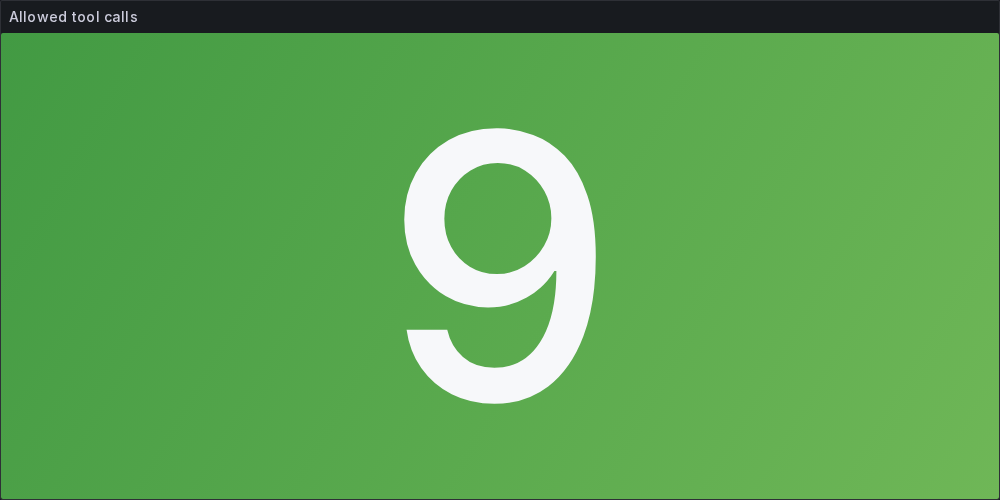
\includegraphics[width=0.4\textwidth]{grafana-allow.png}\hspace{1em}
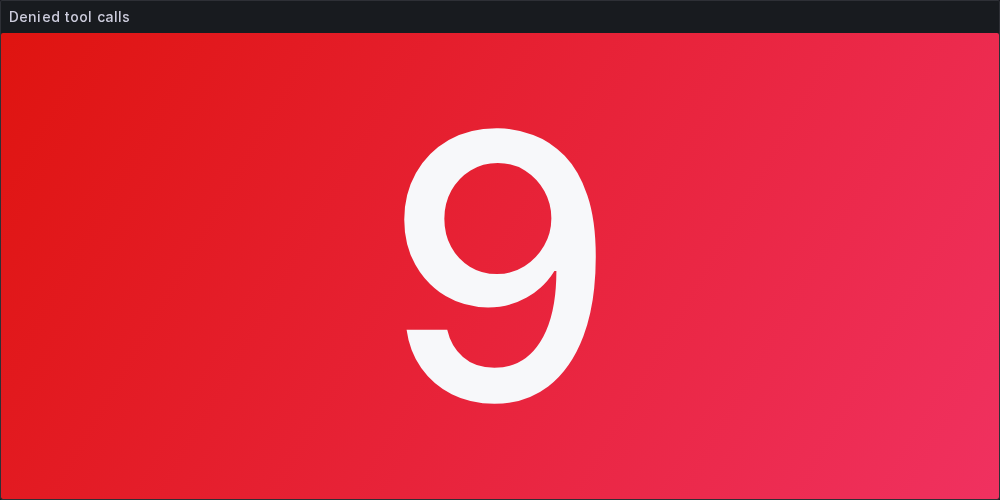
\includegraphics[width=0.4\textwidth]{grafana-deny.png}
\caption{Số lệnh cho phép và bị chặn trên dashboard sau một lượt kiểm thử}\label{fig:allowdeny}\end{figure}

\begingroup\setlength{\emergencystretch}{2em}
\subsection{Đánh giá}
\subsubsection{Đối chiếu mục tiêu}

Bảng~\ref{tab:ch5-goals} tổng hợp số đo của từng yêu cầu. Một yêu cầu được xếp ``Đạt'' khi mọi phép đo đã chạy cho kết quả bằng kỳ vọng và phần cốt lõi có đầu ra đã lưu. Mức ``Một phần'' dành cho trường hợp các phép đo đã chạy đều đạt nhưng vẫn còn tình huống chưa có đầu ra hoặc nằm ngoài phạm vi thử. Tiêu chí này cố ý đặt chặt, đến mức một kết quả đã quan sát được mà không lưu đầu ra cũng không được tính.

\begin{table}[H]\centering\caption{Tổng hợp kết quả đo theo yêu cầu}\label{tab:ch5-goals}
{\singlespacing\renewcommand{\arraystretch}{1.15}\small
\begin{tabularx}{\textwidth}{|c|X|>{\centering\arraybackslash}p{1.7cm}|>{\centering\arraybackslash}p{1.7cm}|>{\centering\arraybackslash}p{1.9cm}|}\hline
\textbf{Mã} & \textbf{Phép đo} & \textbf{Kỳ vọng} & \textbf{Thực tế} & \textbf{Mức đạt} \\ \hline
F1 & Lệnh gọi thành công qua \texttt{/mcp} & 21 & 21 & Đạt \\ \hline
F2 & Tên công cụ đúng tiền tố target & 21 & 21 & Đạt \\ \hline
F3 & Ô ma trận khớp ở \texttt{tools/list} & 210 & 210 & Đạt \\ \hline
S1 & Lệnh ngoài quyền bị chặn & 9 & 9 & Một phần \\ \hline
S2 & Agent có claim \texttt{roles} đúng & 10 & 10 & Đạt \\ \hline
S3 & Lệnh mà backend nhận token gốc & 0 & chưa lưu & Một phần \\ \hline
S4 & Lần thăm dò mạng cho kết quả đúng & 2 & 2 & Một phần \\ \hline
S5 & Lệnh gọi có bản ghi kiểm toán & 18 & 18 & Đạt \\ \hline
O1 & Lần \textit{warm start} đạt kiểm thử (TB áp cấu hình 4,15 giây) & 5 & 5 & Một phần \\ \hline
O2 & Lần đếm allow / deny khớp 9 / 9 & 5 & 5 & Đạt \\ \hline
\end{tabularx}}\end{table}

Sáu yêu cầu đạt, bốn yêu cầu đạt một phần. Ở mọi phép đo đã chạy, giá trị thực tế đều bằng kỳ vọng, và không phép đo nào cho kết quả sai. Bốn yêu cầu đạt một phần cùng chung nguyên nhân là thiếu đầu ra hoặc phạm vi thử hẹp. S1 chưa có đầu ra cho mã 401 và token sai, S3 chưa có đầu ra cho việc xóa token gốc, S4 chưa thăm dò backend ngoài cụm, O1 chưa đo lần dựng từ cụm trống. Mục tiêu chung ở Chương 2 như vậy đạt được ở phần lõi, tức danh mục hợp nhất, phân quyền theo công cụ và cô lập mạng trong cụm. Phần chưa đạt lại rơi vào chiều từ chối của xác thực, cũng là chiều mà kẻ tấn công sẽ thử trước tiên.

\subsubsection{Điểm mạnh}

Điểm mạnh dễ thấy nhất là ma trận kỳ vọng được viết thành dữ liệu và so khớp chính xác. Cùng một ma trận vừa là kết quả mong đợi của kiểm thử đầu cuối, vừa là đầu vào của kiểm thử tĩnh (K9), và lần chạy lại kiểm thử tĩnh ngày 05/11/2026 vẫn đạt với 21 công cụ và 10 agent mà không cần cụm. Bất kỳ thay đổi chính sách nào không kèm cập nhật ma trận sẽ bị bắt ngay trên máy cá nhân, trước khi kịp áp vào cụm.

Điểm mạnh thứ hai nằm ở chỗ việc từ chối diễn ra sớm và ngay tại gateway. 156 trên 210 ô bị ẩn trước khi mô hình kịp chọn công cụ, còn lệnh cố tình gọi bị chặn với \texttt{duration=0ms}, nghĩa là backend không hề nhận được yêu cầu. Thứ ba, mỗi lệnh gọi để lại dấu vết ở nhiều phía độc lập với nhau, gồm phép kiểm ở client, thông tin mock báo lại ở backend, access log ở gateway và dashboard. Các phía này khớp nhau. Và chính vì độc lập, một phía ghi sai sẽ tự lộ ra qua chênh lệch với những phía còn lại.

\subsubsection{Hạn chế}

Hạn chế lớn nhất là bằng chứng và cấu hình hiện tại không hoàn toàn trùng nhau. Toàn bộ bằng chứng được ghi khi năm target đều là mock và các chính sách chỉ chứa quy tắc của agent. Từ đó đến nay, cấu hình đã gộp quy tắc người dùng và agent vào một chính sách, chuyển radar, Spark History và OpenMetadata sang phần mềm thật, lấy \texttt{x-forwarded-user} từ \texttt{preferred\_username} và áp NetworkPolicy cho mọi pod trong namespace backend, nhưng chưa có đầu ra kiểm thử đầu cuối nào trên cấu hình hợp nhất này. Mock lại không gây tác dụng phụ, nên kết quả chưa nói được gì về quyền trên tài nguyên thật như namespace, DAG hay thực thể metadata. Việc đổi token cho OpenMetadata cũng chưa có bằng chứng.

Độ phủ ở bước gọi còn mỏng. 210 ô được so ở bước khám phá, song chỉ 18 lệnh được gọi thật, và chỉ một lệnh thử tách đọc khỏi ghi trên cùng hệ thống. Bộ kiểm thử coi mọi ngoại lệ phía client là ``đã bị chặn'', nên tự nó không phân biệt được một lệnh bị từ chối đúng cách với một lỗi kết nối; mã 400 được xác nhận qua access log và dashboard chứ không qua bộ kiểm thử. Dashboard cũng đếm gộp lệnh thiếu quyền với lệnh gọi sai tên công cụ, hệ quả của việc gateway trả cùng một thông báo \texttt{Unknown tool} cho cả hai. Về vận hành, số đo khởi động mới có năm lần ở tình huống \textit{warm start}. Thời gian dựng từ cụm trống và độ trễ mà gateway thêm vào mỗi lệnh chưa được đo; lớp bọc PowerShell chưa được chạy trực tiếp vì phiên đo chạy bên trong WSL; script dọn dẹp còn để nguyên hai nhóm container compose; và tracing chưa được cấu hình.

\endgroup
% ===== chapters/ch6-ket-luan.tex =====
\chuong{KẾT LUẬN VÀ KIẾN NGHỊ}

\subsection{Kết quả đạt được}

Đề tài đã xây dựng được một hệ thống chứng minh khái niệm trong đó mọi lệnh gọi công cụ của AI Agent đi qua một điểm truy cập MCP duy nhất. Cả 21 công cụ của năm hệ thống gọi được qua gateway (lượt gọi đủ 21 công cụ chạy trước khi bật JWT); mười danh tính agent nhận đúng vai trò trong token, nhìn thấy đúng danh mục công cụ và bị chặn đúng ở công cụ ngoài quyền; Pod ở namespace \texttt{default} không kết nối được tới backend radar, trong khi gateway vẫn kết nối được; và qua năm lần \textit{warm start} liên tiếp, hệ thống áp xong cấu hình trong trung bình 4,15 giây và sẵn sàng phục vụ agent sau khoảng 5,2 giây, kiểm thử phân quyền đạt cả năm lần và access log luôn ghi đúng 9 lệnh cho phép, 9 lệnh bị chặn như ma trận kỳ vọng. Toàn bộ được xây bằng cấu hình các thành phần mã nguồn mở, không có mã gateway riêng.

Trong nhóm, em phụ trách phần đưa AI Agent vào hệ thống một cách kiểm soát được và chứng minh rằng sự kiểm soát đó hoạt động. Cụ thể, em thiết kế danh tính cho mười agent theo luồng client credentials, chia vai trò theo năng lực đọc/ghi trên từng hệ thống thay vì theo chức danh, và cô lập backend bằng NetworkPolicy để agent không thể vượt qua gateway. Em khảo sát khả năng quan sát của agentgateway, tham gia thí nghiệm chồng lấn chính sách, xây dashboard allow/deny trên Grafana và lớp bọc PowerShell cho script khởi động. Toàn bộ phép đo ở Chương~5 do em chạy và lưu đầu ra, từ gọi đủ 21 công cụ, đối chiếu 210 ô ma trận ở \texttt{tools/list}, kiểm tra claim \texttt{roles} của mười agent, đến đo năm lần \textit{warm start} và đối chiếu số đếm allow/deny. Các thành phần nền tảng mà phép đo chạy trên đó, gồm mock server, realm Keycloak, xác thực JWT và bộ quy tắc phân quyền cho người dùng, do thành viên Quân xây dựng; em bổ sung vai trò và quy tắc phân quyền cho agent trên nền đó.

Đối chiếu với mục Đánh giá, mọi phép đo đã chạy đều cho kết quả bằng kỳ vọng. Bốn yêu cầu S1, S3, S4 và O1 dừng ở mức ``Một phần'' vì còn thiếu đầu ra hoặc phạm vi thử còn hẹp: chưa lưu đầu ra cho lỗi 401 và token sai, chưa lưu đầu ra chứng minh token gốc không tới backend, chưa thăm dò backend ngoài cụm, và chưa đo \textit{cold start}. Đây là phần việc em tự đánh giá là còn thiếu và sẽ ưu tiên bổ sung.

\subsection{Bài học kinh nghiệm}

Với định hướng trở thành AI Engineer, bài học lớn nhất em rút ra là mô hình chỉ là một phần của hệ thống AI; phần quyết định agent có được đưa vào vận hành hay không lại nằm ở hạ tầng xung quanh nó. Một agent gọi được công cụ là chưa đủ: doanh nghiệp cần biết agent là ai, được làm gì, đã làm gì, và có thể bị chặn ngay khi vượt quyền. Các câu hỏi đó được trả lời bằng danh tính, phân quyền và nhật ký kiểm toán, không phải bằng prompt.

Bài học thứ hai là thiết kế quyền cho agent khác với cho con người. Vai trò như \texttt{data\_engineer} hợp với một nhân viên nhưng cấp thừa quyền cho agent; chia theo mức đọc và ghi trên từng hệ thống cho phép ghép đúng nhu cầu của từng agent và giữ ma trận kỳ vọng đủ đơn giản để kiểm thử tự động. Đây là nguyên tắc đặc quyền tối thiểu áp dụng cho một loại chủ thể mới, có thể hành động nhanh và nhiều hơn con người.

Bài học thứ ba là phải đánh giá hệ thống bằng thực nghiệm thay vì tin vào tài liệu hay cảm giác. Thí nghiệm chồng lấn chính sách cho thấy chính sách từ chối của agentgateway thắng mọi chính sách cho phép và được đánh giá theo người gọi chứ không theo vai trò, điều tài liệu không nói rõ. Cấu hình sai cũng thường không báo lỗi: header danh tính giả vẫn tới backend khi khối biến đổi bị đặt nhầm chỗ, quy tắc viết theo tên có tiền tố target khiến công cụ bị ẩn, NetworkPolicy không chặn gì nếu cụm thiếu phần mềm mạng phù hợp. Cả ba chỉ lộ ra nhờ kiểm thử đầu cuối so với ma trận kỳ vọng. Tư duy này gần với cách đánh giá mô hình: định nghĩa kết quả kỳ vọng trước, đo trên tập kiểm thử cố định, và chỉ tin vào con số đã lưu.

\subsection{Hướng phát triển}

Ở mức hệ thống, hướng gần nhất là thay mock bằng backend thật và bổ sung phân quyền ở mức tài nguyên, để trả lời câu hỏi ``agent được tác động lên namespace, DAG hay thực thể nào'', đồng thời đo \textit{cold start}, độ trễ của gateway và đưa kiểm thử phân quyền vào quy trình tích hợp liên tục. Tiếp theo là mở rộng sang trường hợp agent hành động thay mặt người dùng, khi quyền hiệu lực phải là giao của quyền agent và quyền người dùng.

Ở mức định hướng cá nhân, em muốn phát triển theo hướng AI Engineer tập trung vào việc đưa agent vào vận hành an toàn: xây agent dùng MCP gọi công cụ thật qua gateway, theo dõi hành vi agent bằng trace và metric để phát hiện vòng lặp gọi công cụ hoặc số lệnh bị chặn tăng bất thường, và xây bộ đánh giá tự động cho agent tương tự ma trận kỳ vọng trong đề tài nhưng mở rộng sang chất lượng câu trả lời. Các kỹ năng cần bổ sung gồm xây dựng agent với LLM, đánh giá mô hình và agent, cùng kiến thức vận hành Kubernetes và bảo mật danh tính đã bắt đầu tích lũy qua đợt kiến tập.

\subsection{Kiến nghị}

Đối với đơn vị, em kiến nghị áp dụng một điểm truy cập MCP duy nhất ngay từ khi đưa AI Agent vào vận hành, cấp cho mỗi agent danh tính riêng và vai trò theo năng lực, tách quyền ghi khỏi quyền đọc, và yêu cầu mọi thay đổi chính sách đi kèm cập nhật ma trận kỳ vọng. Đối với khoa, em kiến nghị bổ sung nội dung thực hành về danh tính và phân quyền cho hệ thống tự động, như OAuth 2.0 giữa máy với máy và kiểm soát truy cập theo vai trò, cùng nội dung về đánh giá và vận hành AI Agent, vì đây là vấn đề doanh nghiệp đang gặp khi triển khai AI vào thực tế.
\heading{TÀI LIỆU THAM KHẢO}
{\setlength{\parskip}{0pt}\printbibliography[heading=none]}
% ===== chapters/phu-luc.tex =====
\heading{PHỤ LỤC}

Các phụ lục trích ý chính của cấu hình và mã nguồn, để người đọc đối chiếu với thiết kế ở Chương 4 mà không phải mở kho mã. Phần lược bỏ được đánh dấu bằng dấu ba chấm. Bản đầy đủ của mọi tệp nằm trong kho mã công khai nêu ở Phụ lục A.

\subsection*{Phụ lục A. Mã nguồn và dữ liệu}
\phantomsection\addcontentsline{toc}{subsection}{Phụ lục A. Mã nguồn và dữ liệu}
\setcounter{table}{0}\renewcommand{\thetable}{A.\arabic{table}}
\needspace{10\baselineskip}\textit{A.1. Kho mã}

\begin{table}[H]\centering
{\singlespacing\renewcommand{\arraystretch}{1.35}\small
\begin{tabularx}{\textwidth}{|>{\raggedright\arraybackslash}p{4cm}|X|}\hline
\textbf{Kho mã nguồn} & \url{https://github.com/QuanVongHuu/MCP-gateway-rbac} \\ \hline
\end{tabularx}}\end{table}

\begin{table}[H]\centering\caption{Vị trí các thành phần trong kho mã}\label{tab:repo}
{\singlespacing\renewcommand{\arraystretch}{1.35}\small
\begin{tabularx}{\textwidth}{|>{\raggedright\arraybackslash}p{5.2cm}|X|}\hline
\textbf{Đường dẫn} & \textbf{Nội dung} \\ \hline
\path{deploy/agentgateway/} & Gateway, HTTPRoute và backend hợp nhất năm target (Phụ lục B.1) \\ \hline
\path{deploy/auth/jwt.yaml} & Xác thực JWT và chuyển tiếp định danh (Phụ lục B.2) \\ \hline
\path{rbac/tool-access.yaml} & Chính sách phân quyền theo công cụ, nguồn sự thật duy nhất (Phụ lục B.3) \\ \hline
\path{deploy/network/backends.yaml} & NetworkPolicy cô lập backend (Phụ lục B.4) \\ \hline
\path{deploy/keycloak/} & Realm, client của agent và script nạp (Phụ lục D) \\ \hline
\path{servers/} & Năm mock MCP server và module dùng chung (Phụ lục C) \\ \hline
\path{tests/} & Kiểm thử tĩnh, kiểm thử đầu cuối và ma trận kỳ vọng \path{tests/expected/agent-tool-access.json} \\ \hline
\path{evidence/} & Đầu ra kiểm thử đã lược bỏ bí mật, dùng ở Chương 5 \\ \hline
\path{ops/}, \path{scripts/} & Script dựng, dọn dẹp và đo thời gian (Phụ lục E) \\ \hline
\path{observability/} & Access log, Loki, Alloy và dashboard Grafana (Phụ lục F) \\ \hline
\end{tabularx}}\end{table}

\needspace{10\baselineskip}\textit{A.2. Ghi chú về dữ liệu}

Mọi dữ liệu trong đề tài đều là dữ liệu thử. Năm mock trả dữ liệu dựng sẵn cho đủ 21 công cụ, và những công cụ mang tính ghi như \texttt{airflow\_trigger\_dag} hay \texttt{radar\_manage\_workload} chỉ trả kết quả mô phỏng, không gây tác dụng phụ nào. Cấu hình hiện tại trỏ ba target radar, OpenMetadata và Spark History sang phần mềm thật chạy cục bộ. Các hệ thống này cũng chỉ chứa dữ liệu thử, bởi radar đọc chính cụm kind của hệ thống, OpenMetadata có người dùng thử cùng một bảng mẫu do script cài đặt tạo ra, còn Spark History đọc ba event log mẫu của dự án gốc. Đề tài không dùng dữ liệu nghiệp vụ của đơn vị kiến tập.

Bằng chứng kiểm thử chỉ lưu đầu ra đã lược bỏ bí mật, nên không chứa client secret, access token hay claim nhạy cảm. Secret của từng agent được sinh thẳng vào Kubernetes Secret, không in ra màn hình, và cấu hình realm chỉ giữ biến giữ chỗ như \texttt{\$\{CLUSTER\_OBSERVER\_AGENT\_SECRET\}}. Tài khoản \texttt{admin}/\texttt{admin} của Keycloak và Grafana, cùng mật khẩu \texttt{password} của người dùng thử, là giá trị mặc định chỉ dành cho môi trường thử cục bộ. Trước khi đưa cấu hình ra khỏi máy cá nhân, các giá trị này phải được thay.

\subsection*{Phụ lục B. Cấu hình gateway}
\phantomsection\addcontentsline{toc}{subsection}{Phụ lục B. Cấu hình gateway}
\needspace{10\baselineskip}\textit{B.1. Backend hợp nhất năm target}

Một backend chứa cả năm target. Giá trị \texttt{Always} của \texttt{prefixMode} tạo tên công cụ dạng \texttt{\{target\}\_\{tool\}}. Bốn target còn lại khai báo giống hệt \texttt{dbt}, chỉ khác tên và địa chỉ.
\par\noindent\begin{minipage}{\linewidth}
\begin{lstlisting}
kind: AgentgatewayBackend
spec:
  mcp:
    prefixMode: Always          # tools appear as {target}_{tool}
    targets:
    - name: dbt
      static: {host: dbt.mcp.svc.cluster.local, port: 80, path: /mcp,
               protocol: StreamableHTTP}
    ...
\end{lstlisting}
\end{minipage}\par
\needspace{10\baselineskip}\textit{B.2. Xác thực JWT và chuyển tiếp định danh}

Chính sách gắn vào Gateway kiểm tra token, ghi đè ba header danh tính bằng claim đã kiểm tra, rồi chuyển token gốc sang header nội bộ \texttt{x-caller-token}. Một chính sách thứ hai, gắn vào backend, xóa header này trước khi yêu cầu rời gateway (S3).
\par\noindent\begin{minipage}{\linewidth}
\begin{lstlisting}
traffic:
  jwtAuthentication:
    mode: Strict
    preserveToken: true
    providers:
    - issuer: http://localhost:8002/realms/mcp
      audiences: [mcp-gateway]
      jwks: {remote: {jwksPath: /realms/mcp/protocol/openid-connect/certs,
                      cacheDuration: "5m", ...}}
  transformation:
    request:
      set:
      - {name: x-forwarded-user,   value: "jwt.preferred_username"}
      - {name: x-agent-id,         value: "has(jwt.azp) ? jwt.azp : ''"}
      - {name: x-forwarded-groups, value: "has(jwt.roles) ? jwt.roles.join(',') : ''"}
      - {name: x-caller-token,     value: 'request.headers["authorization"]'}
      remove: [authorization]
---
# second policy, on the backend: drop the token before it leaves the gateway
backend: {transformation: {request: {remove: [x-caller-token]}}}
\end{lstlisting}
\end{minipage}\par
\needspace{10\baselineskip}\textit{B.3. Phân quyền theo công cụ}

Mọi quy tắc nằm trong một chính sách \texttt{Allow} duy nhất; các biểu thức được nối bằng phép HOẶC, và công cụ không khớp biểu thức nào vừa bị ẩn vừa bị từ chối.
\par\noindent\begin{minipage}{\linewidth}
\begin{lstlisting}
backend:
  mcp:
    authorization:
      action: Allow
      policy:
        matchExpressions:      # expressions are OR-ed
        - 'has(jwt.roles) && "analyst" in jwt.roles
           && mcp.tool.target == "openmetadata"
           && mcp.tool.name in ["search_metadata", "get_entity_details", ...]'
        ...
        - 'has(jwt.roles) && "kube_operator" in jwt.roles
           && mcp.tool.target == "radar" && mcp.tool.name == "manage_workload"'
        - 'has(jwt.roles) && "platform_admin" in jwt.roles'
\end{lstlisting}
\end{minipage}\par
\needspace{10\baselineskip}\textit{B.4. Cô lập mạng}

Chính sách chọn mọi pod trong namespace \texttt{mcp} và chỉ nhận kết nối từ namespace của gateway (S4).
\par\noindent\begin{minipage}{\linewidth}
\begin{lstlisting}
kind: NetworkPolicy
metadata: {name: backends-from-gateway-only, namespace: mcp}
spec:
  podSelector: {}               # every pod in namespace mcp
  policyTypes: [Ingress]
  ingress:
  - from:
    - namespaceSelector:
        matchLabels: {kubernetes.io/metadata.name: agentgateway-system}
\end{lstlisting}
\end{minipage}\par

\subsection*{Phụ lục C. Mock MCP server}
\phantomsection\addcontentsline{toc}{subsection}{Phụ lục C. Mock MCP server}
\setcounter{table}{0}\renewcommand{\thetable}{C.\arabic{table}}
\needspace{10\baselineskip}\textit{C.1. Bộ khung chung}
\par\noindent\begin{minipage}{\linewidth}
\begin{lstlisting}[language=Python]
def new_server(name):
    # stateless + JSON: any gateway replica can serve any request
    return FastMCP(name, host="0.0.0.0", port=8000,
                   stateless_http=True, json_response=True)

def seen(ctx, target, tool, args):
    """Log who called which tool. Never logs the token itself."""
    headers = ctx.request_context.request.headers
    record = {"target": target, "tool": tool, "args": args,
              "x_agent_id": headers.get("x-agent-id"),
              "x_forwarded_user": headers.get("x-forwarded-user"),
              "x_forwarded_groups": headers.get("x-forwarded-groups"),
              "authorization_present": "authorization" in headers}
    if token := bearer(headers):          # non-sensitive claims only
        claims = decode(token)
        record["token"] = {k: claims.get(k) for k in
                           ("iss", "aud", "azp", "sub", "preferred_username", "roles")}
    print(json.dumps(record))
    return record
\end{lstlisting}
\end{minipage}\par
\needspace{10\baselineskip}\textit{C.2. Một công cụ mẫu}
\par\noindent\begin{minipage}{\linewidth}
\begin{lstlisting}[language=Python]
@mcp.tool()
def test(ctx, selector=""):
    """EXECUTE: run dbt data tests. Mock: nothing is run."""
    who = seen(ctx, "dbt", "test", {"selector": selector})
    return {"result": "mock: dbt test -> PASS=17 WARN=1 ERROR=1",
            "seen_by_mock": who}
\end{lstlisting}
\end{minipage}\par
\needspace{10\baselineskip}\textit{C.3. Chức năng của 21 công cụ}
\begin{table}[H]\centering\caption{Chức năng của 21 công cụ}\label{tab:toolfunc}
{\singlespacing\renewcommand{\arraystretch}{1.35}\small
\begin{tabularx}{\textwidth}{|p{2.4cm}|p{3.8cm}|>{\centering\arraybackslash}p{1.5cm}|X|}\hline
\textbf{Target} & \textbf{Công cụ} & \textbf{Loại} & \textbf{Chức năng} \\ \hline
radar & list\_namespaces & Đọc & Liệt kê namespace của cụm \\ \hline
radar & list\_resources & Đọc & Tóm tắt tài nguyên theo loại \\ \hline
radar & get\_pod\_logs & Đọc & Lấy log gần nhất của pod \\ \hline
radar & manage\_workload & Ghi & Khởi động lại, scale, rollback workload \\ \hline
spark-history & list\_applications & Đọc & Liệt kê ứng dụng Spark theo trạng thái \\ \hline
spark-history & get\_stage & Đọc & Chi tiết một stage và chỉ số task \\ \hline
spark-history & get\_job\_bottlenecks & Đọc & Tìm stage chậm, task lệch, lỗi executor \\ \hline
openmetadata & search\_metadata & Đọc & Tìm tài sản dữ liệu theo từ khóa, owner, tag \\ \hline
openmetadata & get\_entity\_details & Đọc & Chi tiết một thực thể theo tên đầy đủ \\ \hline
openmetadata & get\_entity\_lineage & Đọc & Nguồn phía trên và đích phía dưới \\ \hline
openmetadata & patch\_entity & Ghi & Sửa mô tả, tag, owner bằng JSON Patch \\ \hline
dbt & list\_metrics & Đọc & Liệt kê metric của semantic layer \\ \hline
dbt & query\_metrics & Đọc & Truy vấn metric theo chiều \\ \hline
dbt & get\_model\_health & Đọc & Trạng thái chạy, test, độ tươi của model \\ \hline
dbt & get\_lineage & Đọc & Cha và con của một node \\ \hline
dbt & test & Thực thi & Chạy data test theo selector \\ \hline
airflow & list\_dags & Đọc & Liệt kê DAG và lần chạy gần nhất \\ \hline
airflow & get\_dag\_run & Đọc & Trạng thái một lần chạy DAG \\ \hline
airflow & get\_task\_logs & Đọc & Log của một lần thử task \\ \hline
airflow & trigger\_dag & Ghi & Kích hoạt một lần chạy mới \\ \hline
airflow & pause\_dag & Ghi & Tạm dừng DAG \\ \hline
\end{tabularx}}\end{table}

\subsection*{Phụ lục D. Danh tính AI Agent}
\phantomsection\addcontentsline{toc}{subsection}{Phụ lục D. Danh tính AI Agent}
\needspace{10\baselineskip}\textit{D.1. Định nghĩa một client agent}
\par\noindent\begin{minipage}{\linewidth}
\begin{lstlisting}
{"clientId": "cluster-observer-agent",
 "publicClient": false, "serviceAccountsEnabled": true,
 "standardFlowEnabled": false, "directAccessGrantsEnabled": false,
 "secret": "${CLUSTER_OBSERVER_AGENT_SECRET}",
 "protocolMappers": [ audience mcp-gateway, client roles -> claim "roles",
                      hardcoded claim kube_group = "kube_viewer" ]}
...
"users": [{"serviceAccountClientId": "cluster-observer-agent",
           "clientRoles": {"mcp-gateway": ["kube_viewer"]}}, ...]
\end{lstlisting}
\end{minipage}\par
\needspace{10\baselineskip}\textit{D.2. Nạp agent vào realm}
\par\noindent\begin{minipage}{\linewidth}
\begin{lstlisting}[language=bash]
for cid in <clients with a secret>; do   # replace placeholders with real secrets
  sec=$(kubectl get secret agent-client-secrets -o jsonpath={.data.$cid} | base64 -d)
  json=$(jq '(.clients[] | select(.clientId == $c)).secret = $s' ...)
done
# partial import: agent clients and roles only, mcp-gateway untouched
kcadm.sh create partialImport -r mcp  (ifResourceExists: OVERWRITE)
kcadm.sh add-roles --uusername service-account-$cid --rolename $role
\end{lstlisting}
\end{minipage}\par

\subsection*{Phụ lục E. Tự động hóa triển khai}
\phantomsection\addcontentsline{toc}{subsection}{Phụ lục E. Tự động hóa triển khai}
\needspace{10\baselineskip}\textit{E.1. Lớp bọc PowerShell}
\par\noindent\begin{minipage}{\linewidth}
\begin{lstlisting}
$repoDir = (& wsl.exe -d $Distro -- wslpath -u $PSScriptRoot).Trim()
$command = "cd '$repoDir' && bash scripts/up.sh && bash observability/grafana/up.sh"
$stopwatch = [System.Diagnostics.Stopwatch]::StartNew()
& wsl.exe -d $Distro -- bash -lc $command
if ($LASTEXITCODE -ne 0) { throw "Startup failed after $($stopwatch.Elapsed)" }
\end{lstlisting}
\end{minipage}\par
\needspace{10\baselineskip}\textit{E.2. Áp các lớp cấu hình}
\par\noindent\begin{minipage}{\linewidth}
\begin{lstlisting}[language=bash]
set -euo pipefail
kubectl apply -f deploy/agentgateway/Gateway.yaml -f servers/k8s/mocks.yaml ...
kubectl apply -f deploy/keycloak/keycloak.yaml
# setup-realm.sh rebuilds the realm, so only run it when the realm is missing
kcadm.sh get realms/mcp || bash deploy/keycloak/setup-realm.sh
bash scripts/bootstrap-agent-secrets.sh && bash deploy/keycloak/setup-agents.sh
kubectl apply -f deploy/auth/jwt.yaml -f deploy/identity/openmetadata.yaml
kubectl apply -f rbac/tool-access.yaml
kubectl apply -f deploy/network/backends.yaml
kubectl apply -f observability/access-logs/policy.yaml
\end{lstlisting}
\end{minipage}\par
\needspace{10\baselineskip}\textit{E.3. Script dọn dẹp}
\par\noindent\begin{minipage}{\linewidth}
\begin{lstlisting}
& kind delete cluster --name $ClusterName
if ($LASTEXITCODE -ne 0) { Write-Error "Failed to delete ..."; exit $LASTEXITCODE }
\end{lstlisting}
\end{minipage}\par

\subsection*{Phụ lục F. Giám sát allow/deny}
\phantomsection\addcontentsline{toc}{subsection}{Phụ lục F. Giám sát allow/deny}
\needspace{10\baselineskip}\textit{F.1. Bổ sung trường vào access log}
\par\noindent\begin{minipage}{\linewidth}
\begin{lstlisting}
frontend:
  accessLog:
    attributes:
      add:
      - {name: user,       expression: 'has(jwt.preferred_username) ? ... : "anonymous"'}
      - {name: agent_id,   expression: 'has(jwt.azp) ? jwt.azp : ""'}
      - {name: roles,      expression: 'has(jwt.roles) ? jwt.roles : []'}
      - {name: mcp_method, expression: 'has(mcp.methodName) ? mcp.methodName : ""'}
      - {name: mcp_target, expression: 'has(mcp.tool.target) ? mcp.tool.target : ""'}
      - {name: mcp_tool,   expression: 'has(mcp.tool.name) ? mcp.tool.name : ""'}
\end{lstlisting}
\end{minipage}\par
\needspace{10\baselineskip}\textit{F.2. Truy vấn LogQL đếm deny theo vai trò}
\par\noindent\begin{minipage}{\linewidth}
\begin{lstlisting}
sum by (roles) (count_over_time(
  {namespace="agentgateway-system"}
  |~ `mcp.method.name=tools/call` |~ `http.status=400` |~ `Unknown tool`
  | regexp `roles=(?P<roles>\[[^]]*\])` [$__interval]))
\end{lstlisting}
\end{minipage}\par

\subsection*{Phụ lục G. Phân công trong nhóm}
\phantomsection\addcontentsline{toc}{subsection}{Phụ lục G. Phân công trong nhóm}
\setcounter{table}{0}\renewcommand{\thetable}{G.\arabic{table}}
Bảng~\ref{tab:phancong} trình bày phân công theo từng công việc trong kế hoạch của nhóm, kèm thời gian thực hiện. Thời gian chủ yếu theo kế hoạch nên có thể lệch vài ngày so với mốc commit ghi ở Lịch làm việc; cột ``Tham gia'' ghi nhận người hỗ trợ ở công việc mình không phụ trách chính.

\begin{table}[H]\centering\caption{Phân công thực hiện}\label{tab:phancong}
{\singlespacing\renewcommand{\arraystretch}{1.35}\small
\begin{tabularx}{\textwidth}{|>{\raggedright\arraybackslash}X|>{\centering\arraybackslash}p{2.5cm}|>{\centering\arraybackslash}p{2.4cm}|>{\centering\arraybackslash}p{1.6cm}|}\hline
\textbf{Công việc} & \textbf{Thời gian} & \textbf{Phụ trách chính} & \textbf{Tham gia} \\ \hline
Dựng MCP Gateway trên Kubernetes & 30/09 -- 02/10 & \multicolumn{2}{c|}{Cả nhóm} \\ \hline
Mock MCP server cho năm backend (21 công cụ) & 05/10 -- 07/10 & Quân & Huy \\ \hline
Khảo sát khả năng quan sát của agentgateway (log, metric, trace, admin UI) & 05/10 -- 08/10 & Huy & -- \\ \hline
Kiểm chứng gọi đủ 21 công cụ qua gateway & 08/10 & Huy & -- \\ \hline
Thí nghiệm chồng lấn chính sách phân quyền & 08/10 & Quân & Huy \\ \hline
Realm Keycloak, xác thực JWT và quy tắc phân quyền theo công cụ & 07/10 -- 11/10 & Quân & Huy \\ \hline
Dựng và dọn môi trường bằng một lệnh & 06/10 -- 14/10 & \multicolumn{2}{c|}{Quân (bản Linux), Huy (bản Windows)} \\ \hline
README, QUICKSTART và tài liệu dự án & 05/10 -- 14/10 & Quân & Huy \\ \hline
Dashboard allow/deny trên Grafana & 09/10 -- 12/10 & Huy & -- \\ \hline
Kiểm chứng lọc danh mục công cụ theo vai trò & 12/10 & Quân & Huy \\ \hline
Kiểm chứng từ chối lệnh gọi và các trường hợp biên & 13/10 & Quân & Huy \\ \hline
Tổng hợp kết quả giai đoạn 1 vào báo cáo nháp & 12/10 -- 15/10 & Quân & -- \\ \hline
Danh tính AI Agent, cô lập mạng bằng NetworkPolicy và kiểm thử phân quyền theo agent & 22/10 -- 29/10 & Huy & Quân \\ \hline
Đo \textit{warm start} và lưu đầu ra kiểm chứng (benchmark, dashboard) & 05/11 & Huy & -- \\ \hline
Viết báo cáo & -- & \multicolumn{2}{c|}{Chia theo chương, đọc chéo} \\ \hline
\end{tabularx}}\end{table}

\end{document}
